\documentclass[11pt]{article}
\usepackage[margin=2.2cm]{geometry}
\usepackage{amsmath,amssymb}
\usepackage{booktabs,array}
\usepackage{graphicx}
\usepackage{float}
\usepackage{caption}
\usepackage{enumitem}
\usepackage{xcolor}
\usepackage{url}\urlstyle{tt}\setlength{\emergencystretch}{2em}
\usepackage[colorlinks=true,linkcolor=blue!60!black,citecolor=blue!60!black,urlcolor=blue!60!black]{hyperref}
\captionsetup{font=small,labelfont=bf}
\setlist{nosep,leftmargin=1.4em}
% as in draft.tex: shrink a table to the line width only when it is wider
\newsavebox{\fitbox}
\newcommand{\fitcol}[1]{\sbox{\fitbox}{#1}\ifdim\wd\fitbox>\columnwidth\resizebox{\columnwidth}{!}{\usebox{\fitbox}}\else\usebox{\fitbox}\fi}
\newcommand{\note}[1]{\textcolor{red}{[Note: #1]}}
\newcommand{\Copt}{C_{\mathrm{opt}}}
\newcommand{\pending}{\textcolor{red}{(pending)}}

\title{Energy-trajectory view of ADAPT-VQE generator selection\\[2pt]
\large Reproduction of the feature study and new results: findings for updating the draft}
\date{18 October 2026 (cluster rounds 1 and 2; all submitted jobs finished)}

\begin{document}
\maketitle

\begin{abstract}
\noindent
The question of the paper changes from \emph{does the selection find the largest gradient?} to \emph{how many shots does it save without hurting the ADAPT energy trajectory?}
This report collects what two rounds of cluster runs say about that question. The three experiments of the colleague's feature study (correlation of the shared gradient estimates,
confidence level, selection errors) were re-run with her settings, completed for H$_2$O and extended by experiments that vary the size of the selection error and the optimizer tolerance on purpose.
Her deterministic results reproduce; her sampled results reproduce for the selection shots but not for the optimizer evaluation counts, which depend on the build of the Hamiltonian and
on the BFGS tolerance. A selection error inside a fraction $\rho$ of the largest gradient leaves the trajectory unchanged up to $\rho^\ast=0.1$ (LiH), $0.3$ (H$_2$O), $0.5$ (BeH$_2$)
and at least $0.9$ (H$_4$ 2.0~\AA); a tolerance on the \emph{energy lowering} is harmless up to $0.5$ in every system tested, and energy-greedy choices save steps only where the pool leaves room for it (H$_4$ 1.0~\AA, the
stretched 16-qubit window).
The BFGS gradient tolerance of the draft's cost model ($10^{-9}$) is far below what a sampled gradient resolves. At that tolerance the evaluation count depends on the order of near-tied generators and on the build; at $10^{-5}$ and $10^{-3}$ it does not, and the modelled optimization of the complete runs is $2.1$--$3.8$ and $2.9$--$8.1$ times cheaper.
Replaying all recorded runs at those tolerances: lowering the confidence level to 68\% costs no optimization (the rise of H$_4$ 2.0~\AA\ at $10^{-9}$ is path noise); the selection of II-A is $0.1$--$14\%$ of the total ($0.05$--$6\%$ at $10^{-9}$); II-0 and M2 cost $5$--$28\%$ and sequential M1 $1.7$--$4.9$ times more in total on H$_2$O; and the certified selection costs $0.78$--$1.02$ times the cheapest adequate uncertified budget in total shots, although it uses up to $7.1$ times more selection shots.
\end{abstract}

\tableofcontents

%==================================================================================================
\section{Summary and what can go into the draft}

How to read the report: Section~\ref{sec:setup} says what was run; Sections~\ref{sec:repro}--\ref{sec:gtol} give the results, each with the tables in the format of the draft
(\verb|\fitcol|, booktabs; they can be pasted as they are); Section~\ref{sec:draft} lists, section by section, what to change in \texttt{draft.tex}; Section~\ref{sec:open} lists what is
still open. All numbers are read from the stored runs by \texttt{scripts/energy\_findings\_tables.py}; Appendix~\ref{sec:files} gives the files.

\subsection{Findings that can be used now}
\begin{enumerate}
  \item \textbf{The colleague's study reproduces where it is deterministic, and statistically where it is sampled} (Tables~\ref{tab:find_repro}--\ref{tab:find_gate}). 43 of 46 cells of her S1 table and 44 of 54 of her Table~1 agree at the printed precision;
        her median selection shots lie inside the 95\% range of the same statistic over subsets of our runs in 15 of 15 cells, her exact-best shares in 13 of 15. The fast statistics she wrote (\texttt{fastpath.py}) give
        identical selections to the original code on every state tested (H$_2$O equilibrium and stretched, LiH, H$_4$ 2.0~\AA).
  \item \textbf{The shared gradient estimates are uncorrelated for H$_2$O as well} (Table~\ref{tab:find_corr}: 819 and 864 pairs, median $r=0.000$, $\chi=1.000$, $\rho_s\le0.07$): sharing the measurements costs nothing in the comparison of two candidates.
  \item \textbf{The gradient is an imperfect proxy for the energy lowering} (Table~\ref{tab:find_rhomap}). After re-optimizing all parameters the energy-best generator lies inside the $\rho=0.1$ set of the gradient in only $50\%$ (H$_4$ 1.0~\AA), $90\%$,
        $100\%$ (LiH), $47\%$ (H$_2$O eq) and $61\%$ (H$_2$O str) of the states, and the worst generator of that set obtains on average $0.42$, $0.87$, $0.98$, $0.74$ and $0.71$ of the best lowering.
  \item \textbf{ADAPT absorbs gradient-level errors up to a measurable tolerance} (Table~\ref{tab:find_rho}, Fig.~\ref{fig:dose}). With exact gradients and a uniform draw inside the $\rho$-set at every step, the number of steps stays within 3\% of exact ADAPT's up to
        $\rho^\ast=0.1$ (LiH), $0.3$ (H$_2$O eq and stretched), $0.5$ (BeH$_2$), $0.9$ (H$_4$ 2.0~\AA); on H$_4$ 1.0~\AA\ larger $\rho$ gives \emph{fewer} steps. Random ADAPT ($\rho=1$) fails to reach chemical accuracy in all runs on BeH$_2$ and H$_2$O.
        The default $\rho=0.1$ of the paper is the largest value that is harmless on LiH.
  \item \textbf{A tolerance on the energy lowering is safer than one on the gradient} (Table~\ref{tab:find_tau}): drawing from $\{i:\Delta E_i\ge(1-\tau)\max\Delta E\}$ leaves the steps unchanged up to $\tau=0.5$ in every system, where the gradient set at $\rho=0.5$ costs $+49\%$ (LiH), $+13\%$ (H$_2$O eq), $+6\%$ (H$_2$O str).
  \item \textbf{Energy-greedy choices save steps only where the pool leaves room} (Tables~\ref{tab:find_greedy}--\ref{tab:find_window}): H$_4$ 1.0~\AA\ needs 8 instead of 10 steps; on the stretched 16-qubit cc-pVDZ window the energy after 40 steps is $14\%$ lower ($3.23$ against $3.74$~mHa) and
        after 20 steps $24\%$ lower; LiH, BeH$_2$, H$_4$ 2.0~\AA, H$_2$O (STO-3G) and the equilibrium window gain nothing. A choice that needs no extra shots (curvature of the HF state) reproduces the gain on the stretched window only.
  \item \textbf{Selection is a small part of the total, the cheaper selection pays in the total, and certification costs nothing in total shots} (Tables~\ref{tab:find_cost}, \ref{tab:find_cost_tol}, \ref{tab:find_premium}, Figs.~\ref{fig:cost}, \ref{fig:cost_1e-5}). With the modelled optimization cost at $10^{-9}$ the selection of II-A at 95\% is $0.05\%$ (H$_4$ 1.0~\AA), $0.5\%$ (H$_4$ 2.0~\AA), $5.6\%$ (LiH), $0.9\%$ (H$_2$O eq) and $2.3\%$ (H$_2$O str) of the total, and $0.12$--$0.19\%$, $1.2$--$1.9\%$, $11$--$14\%$, $3.3$--$6.8\%$ and $8.2$--$14\%$ at $10^{-5}$ and $10^{-3}$ (replays).
        II-0 and M2 are within $-5$ to $+11\%$ of II-A in total on H$_2$O at $10^{-9}$ and cost $5$--$28\%$ more at the looser tolerances; sequential M1 costs $13\%$ and $66\%$ more at $10^{-9}$ and $1.7$--$4.9$ times as much at the looser ones. The uncertified pilot budgets that reach chemical accuracy in all runs cost $1.2$--$1.6$ times more (all three tolerances), those that reach it in 11 of 12 runs $1.4$--$3.0$ times ($10^{-9}$, $10^{-5}$), because their wrong choices lengthen the trajectory.
        At the cheapest \emph{adequate} budgets of Q10 the certified selection uses $7.1$, $6.4$, $2.1$, $1.0$, $0.5$ and $0.4$ times the selection shots of the uncertified one (H$_4$ 1.0, H$_4$ 2.0, LiH 1.6, LiH 3.0~\AA, H$_2$O eq, H$_2$O str) but costs $0.91$, $0.84$, $0.69$, $0.54$, $0.93$ and $0.83$ times its total at $10^{-9}$, $0.95$, $0.96$, $1.02$, $0.81$, $0.96$ and $0.86$ at $10^{-5}$, and $0.95$, $1.00$, $1.00$, $0.84$, $0.92$ and $0.78$ at $10^{-3}$; the part that is due to the longer trajectories alone is $0.86$--$0.96$. \emph{(At $10^{-9}$ the factors carry the path noise of the optimizer; at $10^{-5}$ and $10^{-3}$ the intervals are about $\pm2$--$12\%$. At $10^{-3}$ the fixed budgets stop being adequate on H$_4$: reach $89\%$ and $95\%$.)}
  \item \textbf{Repairing the small-sample intervals is free at trajectory level} (Table~\ref{tab:find_e5}). On LiH 3.0~\AA\ the default minimum of 50 shots per fold gives a seventh step in $5.6\%$ of 90 trajectories (all five non-$\rho$-good choices are the same generator, shortfall $0.13$--$0.15$);
        a minimum of 200 shots removes them ($0\%$, all choices $\rho$-good) at the same selection cost ($5.08\times10^7$ against $5.16\times10^7$ shots).
  \item \textbf{The BFGS tolerance of the optimizer changes the cost model} (Tables~\ref{tab:find_evals}, \ref{tab:find_gtol_paths}, \ref{tab:find_shares}, \ref{tab:find_cost_tol}, \ref{tab:find_tol_energy}). With the gradient tolerance $10^{-9}$ of \texttt{AdaptSystem.optimize}, the evaluation count of the same generators depends on the order in which they are added
        (LiH: $54$ to $252$ for six generators) and on the build of the Hamiltonian; at $10^{-5}$ and $10^{-3}$ it does neither: every order needs $39$--$40$ and $30$--$31$ evaluations (100 and 200 random orders in the two builds) and the two builds agree on the count of the exact path in all nine comparisons.
        In one build the count of the exact path is $1.3$--$3.3$ times lower at $10^{-5}$ and $1.9$--$6.2$ times lower at $10^{-3}$, and the modelled $\Copt$ of the complete runs is $2.1$--$3.8$ and $2.9$--$8.1$ times lower. The certified runs end at the same energy (within $0.015$~mHa at $10^{-3}$); uncertified runs with poor choices can stall on a plateau at $10^{-3}$.
  \item \textbf{Lowering the confidence level costs no optimization at a consistent tolerance} (Table~\ref{tab:find_conf}). Replaying the sweeps at $10^{-5}$ and $10^{-3}$, $\Copt$ at 68\% is within $-2$ to $+2\%$ of the top level on all five systems (upper interval limits at most $1.05$; H$_4$ 2.0~\AA: $1.01$ [$1.00$, $1.02$] and $1.02$ [$1.00$, $1.03$]), while the selection shots fall by $2.5\times$ (H$_4$ 1.0~\AA), $3.4\times$ (H$_4$ 2.0~\AA), $2.0\times$ (LiH), $1.8\times$ (H$_2$O eq) and $1.6\times$ (H$_2$O str). The rise of $19\%$ that H$_4$ 2.0~\AA\ shows at $10^{-9}$ is path noise of the polishing.
\end{enumerate}

\subsection{What not to quote yet}
\begin{itemize}
  \item Every ratio of an evaluation count or of $\Copt$ to that of the single exact-ADAPT path (her Tables~2 and 3): the reference changes by a factor of 2 between machines and with the tie-break (Table~\ref{tab:find_evals}).
  \item The confidence-level sweep at the tight tolerance alone: at $10^{-9}$ the cost of H$_4$ 2.0~\AA\ rises monotonically from 99\% to 68\% ($+19\%$ [$+6\%$, $+33\%$] in $\Copt$, 48 runs per level) and the other systems have intervals of $\pm10$--$45\%$; this is path noise of the polishing and disappears at $10^{-5}$ and $10^{-3}$ (Table~\ref{tab:find_conf}). Quote ``lowering the confidence costs no optimization'' together with the tolerance.
  \item The curvature-scaled tolerance (Sec.~\ref{sec:greedy}, Tables~\ref{tab:find_nrho}--\ref{tab:find_nrho_window}) as a result of its own: it moves the harmless tolerance outward by one grid step on LiH, BeH$_2$, H$_2$O eq and the equilibrium window and by nothing on H$_4$ and stretched H$_2$O; the grid is $0.1$--$0.2$ wide and the entries have 200 (48) trajectories, so ``harmless up to $R$'' is good to one grid step.
  \item The uncertified baselines at $10^{-3}$: some of their runs stall on plateaus there (Table~\ref{tab:find_tol_energy}); $10^{-5}$ does not show this.
\end{itemize}

%==================================================================================================
\section{What was run}\label{sec:setup}

\paragraph{Systems and selection.} STO-3G, UCCSD pool, Jordan--Wigner: H$_4$ square at 1.0 and 2.0~\AA\ (26 generators; 10 steps, stretched H$_4$ stalls at $3.2$~mHa), LiH at 3.0~\AA\ (92; 6 steps), BeH$_2$ (10 steps), H$_2$O equilibrium (140; 17 steps)
and stretched (18 steps), and the 16-qubit cc-pVDZ window of H$_2$O (core frozen, 8 orbitals; 360 generators; exact ADAPT is still at $5.9$ and $3.7$~mHa after 40 steps, so the energy after a fixed number of steps is the measure). All runs start from Hartree--Fock.
The measured selection is II-A (shared fully commuting contexts, elimination, learned splitting with cross-fitting; sign-aware rule, a priori first radius, per-round intervals, $\rho=0.1$, minimum 50 shots per fold, $\delta=0.05$ unless the confidence level is varied), re-optimization exact.

\paragraph{Cost model.} $\Copt=\sum_k n^{\mathrm{ev}}_k(1+\eta n_k)m_E^{(k)}$ with the BFGS evaluations $n^{\mathrm{ev}}_k$ of the step, $\eta=2$ and $m_E$ the shots of an energy to 1~mHa on sorted-insertion groups of $H$. The BFGS gradient tolerance of \texttt{AdaptSystem.optimize} is $10^{-9}$;
all counts are at that tolerance unless a table says otherwise.

\paragraph{Experiments.} (E0) re-run of the feature study with her settings, completed for H$_2$O (replays of the 36 recorded runs, new measured runs); (E1) selection and optimization together; (E4) the confidence-level sweep with more runs
(48 per level for H$_4$, 24 for LiH, 12 for H$_2$O); (E2, E3) \emph{policy experiments}: ADAPT with exact gradients and exact optimization in which the selection is replaced by a rule that injects an error of a chosen size (uniform draw inside the $\rho$-set of $|g|$, inside the
$\tau$-set of the one-parameter lowering, the worst generator of a set, energy-greedy references), 200 trajectories per random policy, common random numbers over the policies; (E5) complete II-A trajectories on LiH with a minimum of 200 and 400 shots per fold; (E6) the optimizer tolerance: the policy grid at the BFGS gradient tolerances $10^{-5}$ and $10^{-3}$ on the cluster build (200 trajectories per policy), the replay of all recorded sweeps with those tolerances (selections and selection shots kept, optimization re-run) and the replay of the recorded Q10 runs; (E7) the curvature-scaled tolerance at $10^{-5}$ on the cluster build (\texttt{nrho\_random}; six STO-3G systems with 200 trajectories per policy, the two 16-qubit cc-pVDZ windows with 48, the plain gradient set, $\tau=0.3$, the Newton choice and exact ADAPT in the same run).
All shots are simulated and noise-free.

\paragraph{Environments.} The cluster build (Trillium, whole-node jobs) and a local WSL build; they differ in the SCF orbitals of degenerate subspaces, which changes which generators tie and the optimizer's path, so random streams do not carry over between them
(Sec.~\ref{sec:evalenv}). The tolerance tests of Sec.~\ref{sec:gtol} exist in both builds: the policy grid and the replays of the sweeps on the cluster, the path tests and the exact-path counts also in WSL.

%==================================================================================================
\section{Reproduction of the colleague's feature study}\label{sec:repro}

% BEGIN INLINE findings_repro
\begin{table}[!htb]
\centering\small
\caption{Agreement of our re-run of the colleague's study with the numbers of her report. Digit by digit, cells agree when they match at the printed precision; the sampled tables cannot match digit by digit because the random streams do not carry over between builds of the Hamiltonian (Sec.~\ref{sec:evalenv}). The statistical rows test instead whether her statistic lies within the central 95\% of the same statistic over random subsets of her number of runs. Shots and the exact-best share reproduce; the evaluation counts do not.}
\label{tab:find_repro}
\footnotesize\setlength{\tabcolsep}{3.5pt}
\fitcol{%
\begin{tabular}{p{6.2cm}rrp{6.0cm}}
\toprule
Table of her report & cells & agree & what differs \\
\midrule
S1: gradient against one-parameter and full re-optimization lowering, five systems & 46 & 43 & Spearman coefficients, at most $0.03$ (H$_4$ 2.0~\AA: $0.95$ against $0.97$, full $0.83$ against $0.86$) \\
Table 1: correlation of the gradient estimates, five systems, II-0 and II-A & 54 & 44 & pairs 75 against 73 (H$_4$ 2.0~\AA); $r$, $\chi$ and $\rho_s$ within $0.04$ \\
\midrule
Table 2, statistical comparison & \multicolumn{3}{l}{her number inside the 95\% range of $n$-run subsets of our 48 (H$_4$) and 24 (LiH) runs} \\
\quad median selection shots & 15 & 15 & median of hers / ours $= 1.01$ \\
\quad share of selections that were the exact best & 15 & 13 & median of hers / ours $= 1.01$ \\
\quad mean optimizer evaluations (1e-9) & 15 & 9 & median of hers / ours $= 0.90$ \\
\midrule
Table 3, digit by digit (strict tolerance) & 117 & 69 & almost all in the evaluation and $C_\mathrm{opt}$ ratios \\
Table 2, digit by digit (strict tolerance) & 150 & 77 & evaluation counts and their ratios to exact ADAPT; shots differ by the sampling error of 12 runs \\
\bottomrule
\end{tabular}}
\end{table}
% END INLINE findings_repro

% BEGIN INLINE findings_gate
\begin{table}[!htb]
\centering\small
\caption{Gate job: the fast statistics of \texttt{fastpath.py} against the original code of \texttt{LearnedM3}, on the same states and random streams (II-A and, for LiH and H$_4$, also II-0). ``Identical'' means the same generator, rounds, stopping reason, shortfall and shots (relative $10^{-9}$). Replaying the recorded H$_2$O trajectories reproduced their final energies to $0.0$~Ha on the cluster ($1.6\times10^{-13}$~Ha locally).}
\label{tab:find_gate}
\footnotesize\setlength{\tabcolsep}{3.5pt}
\fitcol{%
\begin{tabular}{lllrrr}
\toprule
System & steps tested & methods $\times$ streams & selections compared & identical & time original / fast (s) \\
\midrule
H$_2$O eq & 0 & 1 $\times$ 1 & 1 & 1 & 989 / 519 \\
H$_2$O eq & 7 & 1 $\times$ 1 & 1 & 1 & 1678 / 1094 \\
H$_2$O eq & 14 & 1 $\times$ 1 & 1 & 1 & 2494 / 1661 \\
H$_2$O str & 0 & 1 $\times$ 1 & 1 & 1 & 1001 / 515 \\
H$_2$O str & 9 & 1 $\times$ 1 & 1 & 1 & 2668 / 1997 \\
H$_2$O str & 16 & 1 $\times$ 1 & 1 & 1 & 3021 / 2249 \\
LiH 3.0~\AA & 0, 3, 5 & 2 $\times$ 2 & 12 & 12 & 2115 / 930 \\
H$_4$ 2.0~\AA & 0, 5, 9 & 2 $\times$ 2 & 12 & 12 & 36 / 22 \\
\bottomrule
\end{tabular}}
\end{table}
% END INLINE findings_gate


\paragraph{What reproduces.} Table~S1 of her report (gradient against the energy lowering of a one-parameter move, and after re-optimizing all parameters), including the H$_2$O rows that were open: top-$|g|$ is the best generator in $61\%$ and $68\%$ of the H$_2$O states,
the worst $\rho$-good generator obtains $0.83$ ($0.55$) and $0.76$ ($0.20$) of the best lowering, as in her table; after re-optimization the Spearman correlation of $|g|$ with the lowering is $0.62$ and $0.61$ (new).
Table~\ref{tab:find_corr} is her Table~1 with the H$_2$O rows: the estimates of two gradients from shared data are uncorrelated ($|r|_{90\%}\le0.25$, $\chi=1.00$ in the median); the few strongly correlated pairs are close competitors.

% BEGIN INLINE findings_corr
\begin{table}[!htb]
\centering\small
\caption{Correlation of the gradient estimates from shared measurements against energy lowering (her Table 1), now with the H$_2$O rows: 819 and 864 pairs from the 18 and 19 states of the exact ADAPT trajectories. $r$: correlation of the estimates of $|g|$ of the leader and each challenger; $\chi$: factor by which the shared data change the shots of their comparison; $\rho_s$: Spearman correlation of $r$ with the challenger's lowering over the leader's.}
\label{tab:find_corr}
\footnotesize\setlength{\tabcolsep}{3.5pt}
\fitcol{%
\begin{tabular}{llrrrrrr}
\toprule
System & design & pairs & median $r$ & $|r|_{90\%}$ & $\chi$ median (range) & top pair $r$ / $\chi$ & $\rho_s(r,\Delta E)$ \\
\midrule
H$_4$ 1.0~\AA & II-0 & 74 & -0.02 & 0.15 & 1.02 (0.82--1.23) & -0.01 / 1.01 & -0.12 \\
 & II-A & 74 & -0.01 & 0.15 & 1.01 (0.82--1.17) & -0.03 / 1.03 & -0.00 \\
H$_4$ 2.0~\AA & II-0 & 75 & +0.00 & 0.21 & 1.00 (0.65--1.40) & -0.06 / 1.06 & -0.05 \\
 & II-A & 75 & +0.02 & 0.25 & 0.98 (0.43--1.40) & -0.06 / 1.06 & -0.00 \\
LiH 3.0~\AA & II-0 & 181 & +0.00 & 0.06 & 1.00 (0.76--1.23) & -0.16 / 1.15 & +0.13 \\
 & II-A & 181 & +0.00 & 0.03 & 1.00 (0.84--1.24) & -0.02 / 1.02 & +0.07 \\
H$_2$O eq & II-0 & 819 & +0.00 & 0.03 & 1.00 (0.87--1.19) & +0.00 / 1.00 & +0.06 \\
 & II-A & 819 & +0.00 & 0.03 & 1.00 (0.82--1.13) & +0.00 / 1.00 & +0.07 \\
H$_2$O str & II-0 & 864 & +0.00 & 0.03 & 1.00 (0.75--1.22) & +0.00 / 1.00 & +0.01 \\
 & II-A & 864 & +0.00 & 0.03 & 1.00 (0.92--1.21) & +0.00 / 1.00 & +0.02 \\
\bottomrule
\end{tabular}}
\end{table}
% END INLINE findings_corr


\subsection{Environment and the reference path}\label{sec:evalenv}
The sampled tables cannot match digit by digit because a trajectory is deterministic only in (seed, index, build): the SCF orbitals of degenerate subspaces differ between builds, which changes the Pauli expansion of $H$, which generators tie and the optimizer's path.
The selection side is robust to this (shots, exact-best share), the optimizer side is not. The evaluation count of the single exact-ADAPT path, to which her Tables~2 and 3 normalize, is an arbitrary number: it depends on the tie-break and on the build (Table~\ref{tab:find_evals}), and the mean over random tie-breaks
differs from it by up to a factor of 2 (H$_4$ 1.0~\AA, WSL, $10^{-9}$: $184$ for the lowest-index path against $336$ on average over eight random tie-breaks; LiH: $83$ against $144$).

% BEGIN INLINE findings_evals
\begin{table}[!htb]
\centering\small
\caption{Optimizer evaluations of the exact-ADAPT path (largest $|g|$, ties to the lowest index; BFGS, gradient tolerance in the header, to chemical accuracy) on three machines/builds. At the tight tolerance the count depends on the build of the Hamiltonian (the SCF orbitals of degenerate subspaces differ), so only ratios within one build mean anything; at $10^{-5}$ and $10^{-3}$ the WSL and the cluster build give the same count in 9 of 9 comparisons. In one build the count falls by 1.7--2.9 times (WSL) and 1.3--3.3 times (cluster) at $10^{-5}$ and by 2.5--6.2 (WSL) and 1.9--5.5 (cluster) at $10^{-3}$ (stretched H$_4$ left out). $^\dagger$With the looser tolerance stretched H$_4$ no longer stalls on the gradient test and the run stops on the energy gain after 13 steps instead of 10.}
\label{tab:find_evals}
\footnotesize\setlength{\tabcolsep}{3.5pt}
\fitcol{%
\begin{tabular}{lrrrrrrr}
\toprule
System & her machine & WSL, $10^{-9}$ & cluster, $10^{-9}$ & WSL, $10^{-5}$ & cluster, $10^{-5}$ & WSL, $10^{-3}$ & cluster, $10^{-3}$ \\
\midrule
H$_4$ 1.0~\AA & 285 & 184 & 142 & 110 & 110 & 73 & 73 \\
H$_4$ 2.0~\AA & 242 & 150 & 229 & 89$^\dagger$ & 89$^\dagger$ & 59$^\dagger$ & 59$^\dagger$ \\
LiH 3.0~\AA & 96 & 83 & 115 & 39 & 39 & 30 & 30 \\
BeH$_2$ & -- & 255 & 310 & 105 & 105 & -- & 66 \\
H$_2$O eq & -- & 611 & 517 & 208 & 208 & 99 & 99 \\
H$_2$O str & -- & 720 & 584 & -- & 176 & -- & 107 \\
\bottomrule
\end{tabular}}
\end{table}
% END INLINE findings_evals


\subsection{Which of her conclusions stand}
\begin{itemize}
  \item \emph{Experiment 1} (shared estimates are safe): stands, now for H$_2$O too.
  \item \emph{Experiment 2} (confidence level): the selection shots fall by $2.5\times$ (H$_4$ 1.0~\AA), $3.4\times$ (H$_4$ 2.0~\AA), $2.0\times$ (LiH, 24 runs), $1.8\times$ (H$_2$O eq) and $1.6\times$ (H$_2$O str; 12 runs per level, 99\% to 68\%) from the highest level to 68\%; the steps and the final energy do not change.
        The statement that the optimization cost does \emph{not} grow holds at the tolerances $10^{-5}$ and $10^{-3}$ (every level within $2\%$ of the top one on all five systems) but not at $10^{-9}$, where H$_4$ 2.0~\AA\ rises by $19\%$ with 48 runs per level: the rise is path noise of the polishing (Sec.~\ref{sec:conf}, \ref{sec:gtol}).
  \item \emph{Experiment 3} (errors against optimization cost): stands qualitatively. Small errors do not change the steps; uncertified budgets with large errors lengthen the trajectory (H$_2$O, pilot budgets: $20.8$ steps instead of 17 at $4.2\times10^7$ shots per selection, 27 at $10^7$).
  \item \emph{Table~S1} (gradient against energy): stands; after re-optimization the agreement is weaker than for the one-parameter move (Spearman $0.62$ H$_2$O, $0.64$ H$_4$ 1.0~\AA).
  \item Small points of her text: the abstract says ``2.5--3 times'' where her Table~2 gives $2.3$--$2.9$; ``LiH has 2--3 runs per level'' is too few to resolve any change of the evaluation count (the central 95\% range of the mean of two runs spans a factor of four).
\end{itemize}

%==================================================================================================
\section{Selection and optimization together}\label{sec:cost}

% BEGIN INLINE findings_cost
\begin{table}[!htb]
\centering\small
\caption{Selection and optimization together: median total shots (selection plus modelled $C_\mathrm{opt}$, $\eta=2$, BFGS tolerance $10^{-9}$) of complete measured runs relative to II-A at 95\%. Selection share: selection shots over the total. Reach: share of runs that reach chemical accuracy (a run that does not is stopped at ten steps above exact ADAPT's count, so its total is a lower bound). The fixed budgets are the uncertified pilot-allocation selections. II-A rows: 48 (H$_4$), 24 (LiH) runs per level from the larger sets, 12 (H$_2$O eq) at 99, 90 and 68\%, 36 at 95\%; the other methods are the 36 recorded runs (H$_2$O), 12 runs per budget. At this tolerance a median total fluctuates by $\pm20$--$30\%$ between sets of 24 runs (tie-order noise of the optimizer), by $\pm7\%$ for 36 runs of H$_2$O.}
\label{tab:find_cost}
\footnotesize\setlength{\tabcolsep}{3.5pt}
\fitcol{%
\begin{tabular}{llrrrrr}
\toprule
System & method & runs & steps & reach & selection share & total / II-A (95\%) \\
\midrule
H$_4$ 1.0~\AA & II-A 99\% & 48 & 10.0 & 100\% & 0.078\% & 0.90 \\
 & II-A 97\% & 48 & 10.0 & 100\% & 0.059\% & 0.96 \\
 & II-A 95\% & 48 & 10.0 & 100\% & 0.051\% & 1.00 \\
 & II-A 90\% & 48 & 10.0 & 100\% & 0.041\% & 1.07 \\
 & II-A 80\% & 48 & 10.0 & 100\% & 0.034\% & 1.07 \\
 & II-A 68\% & 48 & 10.0 & 100\% & 0.026\% & 1.06 \\
 & fixed $1.0\times10^{3}$ (pilot) & 12 & 20.0 & 0\% & 0.0016\% & 0.62 \\
 & fixed $3.2\times10^{3}$ (pilot) & 12 & 16.5 & 92\% & 0.00083\% & 2.98 \\
 & fixed $1.0\times10^{4}$ (pilot) & 12 & 12.1 & 100\% & 0.0038\% & 1.51 \\
\midrule
H$_4$ 2.0~\AA & II-A 99\% & 48 & 10.0 & 100\% & 0.72\% & 1.00 \\
 & II-A 97\% & 48 & 10.0 & 100\% & 0.52\% & 1.02 \\
 & II-A 95\% & 48 & 10.0 & 100\% & 0.46\% & 1.00 \\
 & II-A 90\% & 48 & 10.0 & 100\% & 0.28\% & 1.02 \\
 & II-A 80\% & 48 & 10.0 & 100\% & 0.26\% & 1.02 \\
 & II-A 68\% & 48 & 10.0 & 100\% & 0.19\% & 1.09 \\
\midrule
LiH 3.0~\AA & II-A 99\% & 24 & 6.0 & 100\% & 10\% & 0.76 \\
 & II-A 97\% & 24 & 6.0 & 100\% & 5.5\% & 1.01 \\
 & II-A 95\% & 24 & 6.0 & 100\% & 5.6\% & 1.00 \\
 & II-A 90\% & 24 & 6.0 & 100\% & 4.4\% & 0.99 \\
 & II-A 80\% & 24 & 6.0 & 100\% & 4.4\% & 0.98 \\
 & II-A 68\% & 24 & 6.0 & 100\% & 3.9\% & 1.00 \\
\midrule
H$_2$O eq & II-A 99\% & 12 & 17.0 & 100\% & 1.2\% & 0.86 \\
 & II-A 95\% & 36 & 17.0 & 100\% & 0.89\% & 1.00 \\
 & II-A 90\% & 12 & 17.0 & 100\% & 0.84\% & 0.85 \\
 & II-A 68\% & 12 & 17.0 & 100\% & 0.65\% & 0.89 \\
 & II-0 & 36 & 17.0 & 100\% & 2.2\% & 0.95 \\
 & M2 & 36 & 17.0 & 100\% & 2.2\% & 1.01 \\
 & M1 seq., & 36 & 17.0 & 100\% & 18\% & 1.13 \\
 & fixed $1.0\times10^{7}$ (pilot) & 12 & 27.0 & 0\% & 0.095\% & 2.37 \\
 & fixed $2.4\times10^{7}$ (pilot) & 12 & 25.8 & 25\% & 0.22\% & 2.40 \\
 & fixed $4.2\times10^{7}$ (pilot) & 12 & 20.8 & 100\% & 0.45\% & 1.55 \\
 & fixed $5.6\times10^{7}$ (pilot) & 12 & 19.2 & 100\% & 0.66\% & 1.36 \\
\midrule
H$_2$O str & II-A 99\% & 12 & 18.0 & 100\% & 2.6\% & 1.06 \\
 & II-A 95\% & 36 & 18.0 & 100\% & 2.3\% & 1.00 \\
 & II-A 90\% & 12 & 18.0 & 100\% & 2.1\% & 1.00 \\
 & II-A 68\% & 12 & 18.0 & 100\% & 1.7\% & 1.04 \\
 & II-0 & 36 & 18.0 & 100\% & 6.4\% & 1.05 \\
 & M2 & 36 & 18.0 & 100\% & 6.4\% & 1.11 \\
 & M1 seq., & 36 & 18.0 & 100\% & 42\% & 1.66 \\
 & fixed $3.2\times10^{7}$ (pilot) & 12 & 28.0 & 0\% & 0.31\% & 2.47 \\
 & fixed $1.0\times10^{8}$ (pilot) & 12 & 27.4 & 8\% & 0.89\% & 2.70 \\
 & fixed $1.8\times10^{8}$ (pilot) & 12 & 23.9 & 92\% & 2.2\% & 1.63 \\
 & fixed $3.2\times10^{8}$ (pilot) & 12 & 19.5 & 100\% & 4.2\% & 1.22 \\
\bottomrule
\end{tabular}}
\end{table}
% END INLINE findings_cost


\begin{figure}[!ht]
  \centering
  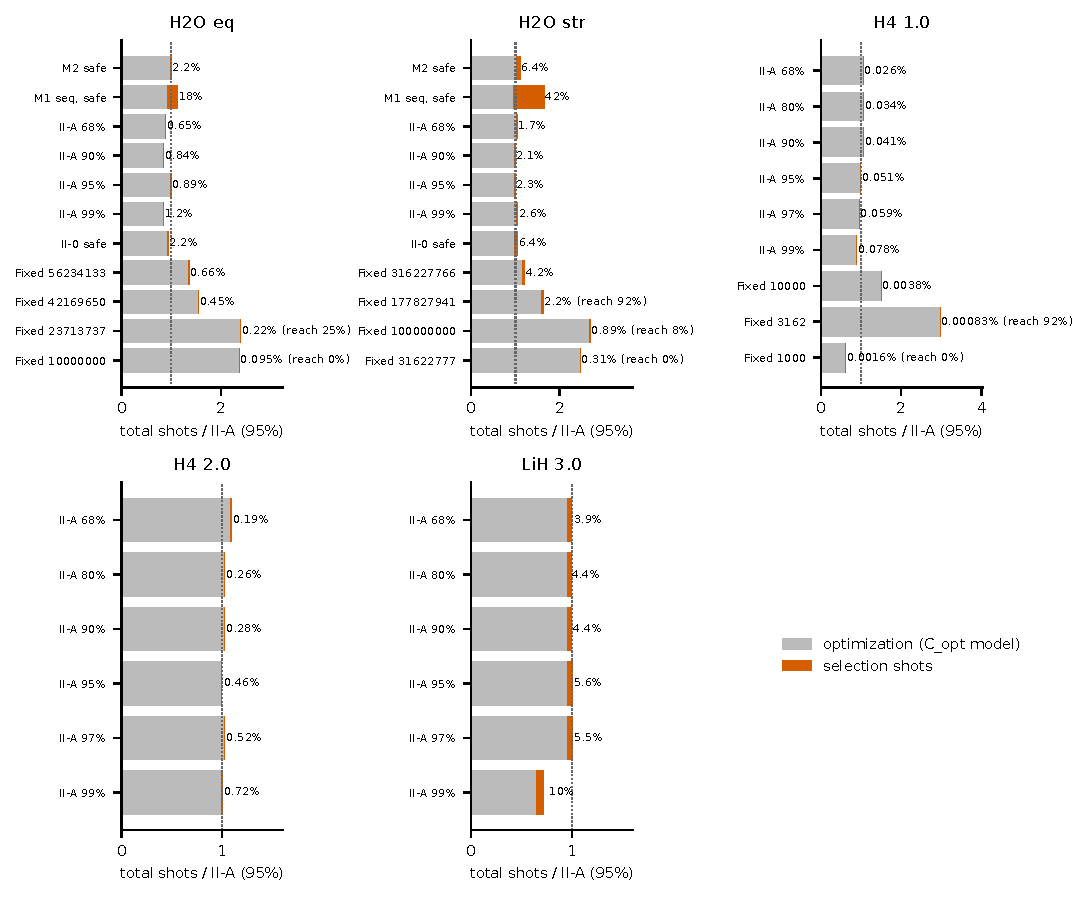
\includegraphics[width=0.92\textwidth]{figures/findings_cost_totals.pdf}
  \caption{Table~\ref{tab:find_cost} as bars: the median total of each method relative to II-A at 95\% (grey: modelled optimization; orange: selection shots), with the selection share and, below 95\%, the share of runs that reach chemical accuracy.}
  \label{fig:cost}
\end{figure}

\paragraph{Reading.} After compression the selection of II-A at 95\% is $0.05\%$ (H$_4$ 1.0~\AA), $0.5\%$ (H$_4$ 2.0~\AA), $5.6\%$ (LiH), $0.9\%$ (H$_2$O eq) and $2.3\%$ (H$_2$O str) of the modelled total; over all confidence levels it is $0.03$--$0.7\%$ (H$_4$), $3.9$--$10\%$ (LiH) and $0.6$--$1.2\%$ (H$_2$O eq). Hence II-A, II-0 and M2 are within $-5$ to $+11\%$ in total on H$_2$O (medians; $-4$ to $+6\%$ in means, with a standard error of $2$--$3\%$ each) although II-A uses $2.3$--$3.1$ times fewer selection shots than II-0 and M2.
Sequential M1 costs $+13\%$ (eq) and $+66\%$ (str) (means: $+14\%$, $+62\%$). Uncertified pilot budgets that reach chemical accuracy in all 12 runs cost $1.2$--$1.6$ times the total of II-A ($1.51$ on H$_4$ 1.0~\AA, $1.55$ and $1.36$ on H$_2$O eq, $1.22$ on H$_2$O str), those that reach it in 11 of 12 runs $3.0$ (H$_4$ 1.0~\AA) and $1.6$ (H$_2$O str), and the budgets that do not reach it $2.4$--$2.7$ times on H$_2$O (their total is then a lower bound).
All numbers of this table are at the tight tolerance $10^{-9}$ of the draft; the shares scale with the optimization cost and grow when the optimizer needs fewer evaluations (next table and paragraph).

% BEGIN INLINE findings_cost_tol
\begin{table}[!htb]
\centering\small
\caption{Selection and optimization together at three BFGS gradient tolerances: share of the selection in the total and median total relative to II-A at 95\%, by replaying the recorded runs (selections and selection shots kept, optimization re-run; cluster build; the other methods are the 36 recorded runs of H$_2$O, the fixed budgets 12 runs each). Reach is the share of runs that end at chemical accuracy at the tight and at the loosest tolerance; a run that does not reach it is stopped at ten steps above exact ADAPT's count, so its total is a lower bound. At the looser tolerances the optimization is cheaper and every difference in selection shots weighs more: II-0 and M2 cost more than II-A, sequential M1 several times as much.}
\label{tab:find_cost_tol}
\footnotesize\setlength{\tabcolsep}{3.5pt}
\fitcol{%
\begin{tabular}{llrrrrrrrr}
\toprule
System & method & runs & reach, $10^{-9}$ / $10^{-3}$ & share, $10^{-9}$ & $10^{-5}$ & $10^{-3}$ & total / II-A (95\%), $10^{-9}$ & $10^{-5}$ & $10^{-3}$ \\
\midrule
H$_4$ 1.0~\AA & II-A 95\% & 48 & 100\% / 100\% & 0.051\% & 0.12\% & 0.19\% & 1.00 & 1.00 & 1.00 \\
 & fixed $1.0\times10^{3}$ (pilot) & 12 & 0\% / 0\% & 0.0016\% & 0.0026\% & 0.0042\% & 0.62 & 0.89 & 0.83 \\
 & fixed $3.2\times10^{3}$ (pilot) & 12 & 92\% / 50\% & 0.00083\% & 0.0027\% & 0.0057\% & 2.98 & 2.18 & 1.60 \\
 & fixed $1.0\times10^{4}$ (pilot) & 12 & 100\% / 75\% & 0.0038\% & 0.011\% & 0.019\% & 1.51 & 1.20 & 1.07 \\
\midrule
H$_4$ 2.0~\AA & II-A 95\% & 48 & 100\% / 100\% & 0.46\% & 1.2\% & 1.9\% & 1.00 & 1.00 & 1.00 \\
\midrule
LiH 3.0~\AA & II-A 95\% & 24 & 100\% / 100\% & 5.6\% & 11\% & 14\% & 1.00 & 1.00 & 1.00 \\
\midrule
H$_2$O eq & II-A 95\% & 36 & 100\% / 100\% & 0.89\% & 3.3\% & 6.8\% & 1.00 & 1.00 & 1.00 \\
 & II-0 & 36 & 100\% / 100\% & 2.2\% & 7.3\% & 14\% & 0.95 & 1.04 & 1.09 \\
 & M2 & 36 & 100\% / 100\% & 2.2\% & 7.8\% & 15\% & 1.01 & 1.05 & 1.10 \\
 & M1 seq., & 36 & 100\% / 100\% & 18\% & 44\% & 63\% & 1.13 & 1.73 & 2.52 \\
 & fixed $1.0\times10^{7}$ (pilot) & 12 & 0\% / 0\% & 0.095\% & 0.6\% & 1.1\% & 2.37 & 1.37 & 1.61 \\
 & fixed $2.4\times10^{7}$ (pilot) & 12 & 25\% / 25\% & 0.22\% & 1.2\% & 2.1\% & 2.40 & 1.68 & 1.91 \\
 & fixed $4.2\times10^{7}$ (pilot) & 12 & 100\% / 100\% & 0.45\% & 1.9\% & 3.6\% & 1.55 & 1.40 & 1.50 \\
 & fixed $5.6\times10^{7}$ (pilot) & 12 & 100\% / 100\% & 0.66\% & 2.7\% & 5.3\% & 1.36 & 1.21 & 1.27 \\
\midrule
H$_2$O str & II-A 95\% & 36 & 100\% / 100\% & 2.3\% & 8.2\% & 14\% & 1.00 & 1.00 & 1.00 \\
 & II-0 & 36 & 100\% / 100\% & 6.4\% & 21\% & 31\% & 1.05 & 1.16 & 1.26 \\
 & M2 & 36 & 100\% / 100\% & 6.4\% & 21\% & 33\% & 1.11 & 1.17 & 1.28 \\
 & M1 seq., & 36 & 100\% / 100\% & 42\% & 73\% & 82\% & 1.66 & 3.36 & 4.91 \\
 & fixed $3.2\times10^{7}$ (pilot) & 12 & 0\% / 0\% & 0.31\% & 2.3\% & 3.2\% & 2.47 & 1.18 & 1.40 \\
 & fixed $1.0\times10^{8}$ (pilot) & 12 & 8\% / 8\% & 0.89\% & 5.4\% & 8.2\% & 2.70 & 1.57 & 1.70 \\
 & fixed $1.8\times10^{8}$ (pilot) & 12 & 92\% / 92\% & 2.2\% & 9.3\% & 14\% & 1.63 & 1.36 & 1.50 \\
 & fixed $3.2\times10^{8}$ (pilot) & 12 & 100\% / 100\% & 4.2\% & 15\% & 23\% & 1.22 & 1.20 & 1.31 \\
\bottomrule
\end{tabular}}
\end{table}
% END INLINE findings_cost_tol


\paragraph{At the looser tolerances} (Table~\ref{tab:find_cost_tol}). The modelled optimization of the complete runs is $2.1$--$3.8$ times cheaper at $10^{-5}$ and $2.9$--$8.1$ times cheaper at $10^{-3}$ (medians of the replays), so the selection weighs more: its share for II-A at 95\% is $0.12$--$0.19\%$ (H$_4$ 1.0~\AA), $1.2$--$1.9\%$ (H$_4$ 2.0~\AA), $11$--$14\%$ (LiH), $3.3$--$6.8\%$ (H$_2$O eq) and $8.2$--$14\%$ (H$_2$O str), against $0.05$--$5.6\%$ at $10^{-9}$.
Every difference in selection shots now shows in the total: II-0 and M2, which use $2.3$--$3.1$ times more selection shots than II-A, cost $5$--$17\%$ ($10^{-5}$) and $9$--$28\%$ ($10^{-3}$) more in total on H$_2$O, and sequential M1 costs $1.7$ and $3.4$ times ($10^{-5}$), $2.5$ and $4.9$ times ($10^{-3}$) as much on H$_2$O eq and str. The uncertified pilot budgets that reach chemical accuracy in all runs cost $1.2$--$1.4$ times ($10^{-5}$) and $1.3$--$1.5$ times ($10^{-3}$) the total of II-A; at $10^{-3}$ some runs of the H$_4$ 1.0~\AA\ pilot budgets stall (reach $75\%$ and $50\%$ instead of $100\%$ and $92\%$, Table~\ref{tab:find_tol_energy}).
Lowering the confidence from 99\% to 68\% saves $7\%$ and $9\%$ of the total on LiH, $2\%$ and $3\%$ on H$_2$O eq, $4\%$ and $6\%$ on H$_2$O str and $1\%$ on H$_4$ 2.0~\AA\ at $10^{-5}$ and $10^{-3}$ (on H$_4$ 1.0~\AA\ nothing within the noise of the medians); the saving cannot exceed the selection share, which the orange parts of Fig.~\ref{fig:cost_1e-5} show.

\begin{figure}[!ht]
  \centering
  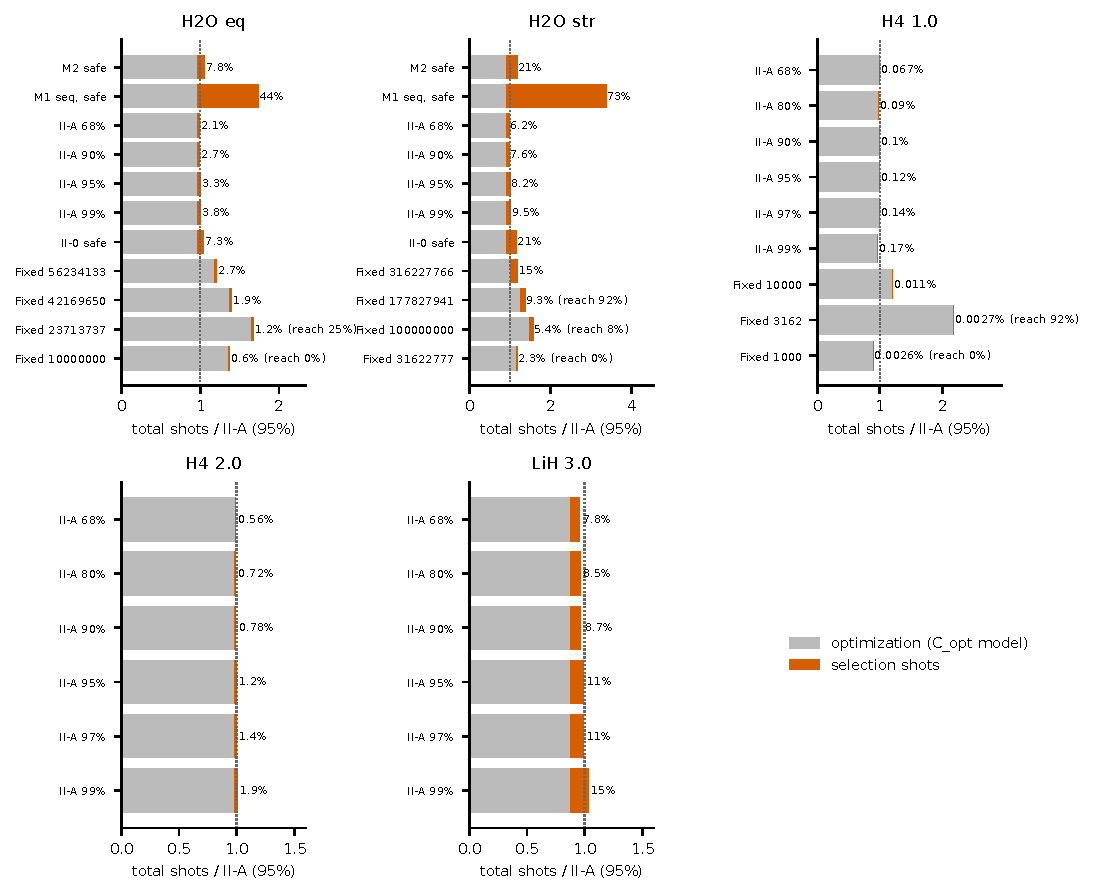
\includegraphics[width=0.92\textwidth]{figures/findings_cost_totals_1e-5.pdf}
  \caption{As Fig.~\ref{fig:cost} at the BFGS gradient tolerance $10^{-5}$ (replay of the recorded runs, cluster build): median total of each method relative to II-A at 95\% (grey: modelled optimization; orange: selection shots), with the selection share and, below 95\%, the share of runs that reach chemical accuracy.}
  \label{fig:cost_1e-5}
\end{figure}

% BEGIN INLINE findings_premium
\begin{table}[!htb]
\centering\small
\caption{Certification premium of Q10 in selection shots and in total shots. The fixed budget is the cheapest adequate one of Q10 (designed allocation: at least 95\% of the trajectories reach chemical accuracy within one step of exact ADAPT's count); II-A is the certified selection at 95\%, both from the recorded Phase~4 runs with their optimization recomputed ($C_\mathrm{opt}$ model, $\eta=2$, BFGS gradient tolerance $10^{-9}$ as in the draft, and $10^{-5}$ and $10^{-3}$ by replaying the recorded choices). The premium is the ratio II-A over fixed. Selection-only premium as in the draft; in total shots the premium is the ratio of the medians of the sums (bootstrap 95\% interval in brackets), where the fixed budget pays for its longer trajectories. The last column is the ratio of the mean numbers of steps, the part of the premium that is due to the longer trajectories alone; at $10^{-9}$ the rest is mostly the path dependence of the optimizer's evaluation count (Sec.~\ref{sec:gtol}), which is larger for the runs with more near-tied choices. The designed fixed budgets are adequate at $10^{-9}$ by construction; at the looser tolerances some of their runs stall on a plateau, and the share that reaches chemical accuracy falls to 89\% (H$_4$ 1.0~\AA, $10^{-3}$), 95\% (H$_4$ 2.0~\AA, $10^{-3}$) (II-A: all runs).}
\label{tab:find_premium}
\footnotesize\setlength{\tabcolsep}{3.5pt}
\fitcol{%
\begin{tabular}{llrrrrrr}
\toprule
System & fixed: budget per step / selection shots & steps, fixed (II-A) & premium, selection only & premium, total, $10^{-9}$ & $10^{-5}$ & $10^{-3}$ & from steps alone \\
\midrule
H$_4$ 1.0~\AA & $1.3\times10^{4}$ / $1.5\times10^{5}$ & 10.93 (10.00) & 7.1 & 0.91 (0.81--1.03) & 0.95 (0.93--0.97) & 0.95 (0.93--0.97) & 0.92 \\
H$_4$ 2.0~\AA & $1.3\times10^{5}$ / $1.5\times10^{6}$ & 11.00 (10.00) & 6.4 & 0.84 (0.70--1.28) & 0.96 (0.95--1.01) & 1.00 (0.97--1.02) & 0.91 \\
LiH 1.6~\AA & $3.2\times10^{6}$ / $1.6\times10^{7}$ & 5.83 (5.00) & 2.1 & 0.69 (0.64--1.26) & 1.02 (0.95--1.10) & 1.00 (0.97--1.12) & 0.86 \\
LiH 3.0~\AA & $7.5\times10^{6}$ / $5.2\times10^{7}$ & 6.73 (6.07) & 1.0 & 0.54 (0.39--0.75) & 0.81 (0.75--0.91) & 0.84 (0.77--0.96) & 0.90 \\
H$_2$O eq & $1.3\times10^{8}$ / $2.3\times10^{9}$ & 17.72 (17.00) & 0.5 & 0.93 (0.84--1.01) & 0.96 (0.88--0.98) & 0.92 (0.80--0.94) & 0.96 \\
H$_2$O str & $4.2\times10^{8}$ / $7.6\times10^{9}$ & 18.78 (18.00) & 0.4 & 0.83 (0.79--0.96) & 0.86 (0.81--0.87) & 0.78 (0.73--0.80) & 0.96 \\
\bottomrule
\end{tabular}}
\end{table}
% END INLINE findings_premium


\paragraph{Q10 in total shots.} The draft's certification premium counts selection shots only. Table~\ref{tab:find_premium} adds the optimization of the same runs. The cheapest \emph{adequate} fixed budgets of Q10 (at least 95\% of the trajectories within one step of exact ADAPT's count)
still lengthen the trajectories by $0.7$ to $1.0$ steps on average ($+4\%$ on H$_2$O to $+17\%$ on LiH 1.6~\AA), which the premium in selection shots does not see: the certified selection uses $0.4$ to $7.1$ times the selection shots of the fixed budget and costs $0.91$, $0.84$, $0.69$, $0.54$, $0.93$ and $0.83$ times its total at $10^{-9}$ ($7$ to $46\%$ cheaper, with intervals of $\pm8$--$40\%$ that carry the path noise of the optimizer),
$0.95$, $0.96$, $1.02$, $0.81$, $0.96$ and $0.86$ at $10^{-5}$ and $0.95$, $1.00$, $1.00$, $0.84$, $0.92$ and $0.78$ at $10^{-3}$ (intervals about $\pm2$--$12\%$): in total shots certification is not dearer (at most $+2\%$, inside the interval, on LiH 1.6~\AA) and up to $22\%$ cheaper. The part explained by the extra steps alone is $0.86$--$0.96$; at the looser tolerances the extra selection shots eat part of that gain because the selection is a larger share of the total, on LiH 1.6~\AA\ all of it.
At $10^{-3}$ the budgets that are adequate at $10^{-9}$ are no longer adequate on H$_4$ (reach $89\%$ on H$_4$ 1.0~\AA, $95\%$ on H$_4$ 2.0~\AA; II-A $100\%$). The statement that survives every tolerance is ``not dearer in total, and up to $22\%$ cheaper'', not the factors of the $10^{-9}$ column.

%==================================================================================================
\section{Confidence level and the trajectory}\label{sec:conf}

% BEGIN INLINE findings_conf
\begin{table}[!htb]
\centering\small
\caption{Confidence level of the selection against the optimization cost of the complete run (II-A, sign-aware rule, a priori start, $\rho=0.1$): $C_\mathrm{opt}$ relative to the highest level of the system, at the BFGS gradient tolerance $10^{-9}$ of the draft and, by replaying the recorded choices, at $10^{-5}$ and $10^{-3}$ (cluster build). Runs: 48 per level for H$_4$, 24 for LiH; H$_2$O: 12 at each of 99, 90 and 68\% (new) and the 36 recorded runs at 95\% replayed with their optimization (the only level that was not run afresh). ``Top'' is the highest level of the system and the interval is a bootstrap interval of the ratio of the means. At $10^{-9}$ the cost of H$_4$ 2.0~\AA\ rises monotonically as the confidence falls; at $10^{-5}$ and $10^{-3}$ no level differs from the top one by more than a few percent (Sec.~\ref{sec:gtol}).}
\label{tab:find_conf}
\footnotesize\setlength{\tabcolsep}{3.5pt}
\fitcol{%
\begin{tabular}{lrrrrlll}
\toprule
System & conf. & runs & selection shots & steps & $C_\mathrm{opt}$ / top [95\% CI], $10^{-9}$ & $10^{-5}$ & $10^{-3}$ \\
\midrule
H$_4$ 1.0~\AA & 99\% & 48 & $1.5\times10^{6}$ & 10.00 & 1.00 [0.87, 1.15] & 1.00 [0.99, 1.01] & 1.00 [0.99, 1.01] \\
 & 97\% & 48 & $1.2\times10^{6}$ & 10.00 & 1.03 [0.91, 1.17] & 1.01 [1.00, 1.02] & 1.01 [1.00, 1.01] \\
 & 95\% & 48 & $1.1\times10^{6}$ & 10.00 & 1.01 [0.90, 1.14] & 1.01 [1.00, 1.02] & 1.00 [0.99, 1.01] \\
 & 90\% & 48 & $9.3\times10^{5}$ & 10.00 & 1.05 [0.93, 1.18] & 1.02 [1.01, 1.03] & 1.01 [1.00, 1.02] \\
 & 80\% & 48 & $7.8\times10^{5}$ & 10.00 & 1.11 [0.97, 1.26] & 1.01 [1.00, 1.02] & 1.01 [1.00, 1.02] \\
 & 68\% & 48 & $5.9\times10^{5}$ & 10.00 & 1.07 [0.94, 1.21] & 1.02 [1.01, 1.03] & 1.01 [1.00, 1.02] \\
\midrule
H$_4$ 2.0~\AA & 99\% & 48 & $1.5\times10^{7}$ & 10.00 & 1.00 [0.90, 1.12] & 1.00 [0.99, 1.01] & 1.00 [0.99, 1.01] \\
 & 97\% & 48 & $1.1\times10^{7}$ & 10.00 & 1.03 [0.92, 1.14] & 1.00 [0.99, 1.00] & 1.01 [1.00, 1.02] \\
 & 95\% & 48 & $9.6\times10^{6}$ & 10.00 & 1.09 [0.97, 1.24] & 1.00 [1.00, 1.01] & 1.01 [1.00, 1.02] \\
 & 90\% & 48 & $6.1\times10^{6}$ & 10.00 & 1.13 [1.00, 1.26] & 1.01 [1.00, 1.02] & 1.01 [0.99, 1.02] \\
 & 80\% & 48 & $5.6\times10^{6}$ & 10.00 & 1.17 [1.03, 1.32] & 1.01 [1.00, 1.02] & 1.00 [0.99, 1.02] \\
 & 68\% & 48 & $4.4\times10^{6}$ & 10.00 & 1.19 [1.06, 1.33] & 1.01 [1.00, 1.02] & 1.02 [1.00, 1.03] \\
\midrule
LiH 3.0~\AA & 99\% & 24 & $7.2\times10^{7}$ & 6.04 & 1.00 [0.64, 1.55] & 1.00 [0.95, 1.05] & 1.00 [0.95, 1.05] \\
 & 97\% & 24 & $5.1\times10^{7}$ & 6.04 & 1.05 [0.69, 1.59] & 1.00 [0.95, 1.05] & 0.99 [0.95, 1.03] \\
 & 95\% & 24 & $5.1\times10^{7}$ & 6.04 & 1.00 [0.66, 1.51] & 1.00 [0.95, 1.05] & 1.00 [0.95, 1.04] \\
 & 90\% & 24 & $4.0\times10^{7}$ & 6.00 & 0.96 [0.65, 1.44] & 0.98 [0.95, 1.00] & 0.98 [0.95, 1.01] \\
 & 80\% & 24 & $3.9\times10^{7}$ & 6.00 & 0.92 [0.62, 1.38] & 0.98 [0.95, 1.00] & 0.98 [0.94, 1.00] \\
 & 68\% & 24 & $3.5\times10^{7}$ & 6.04 & 1.14 [0.77, 1.71] & 1.00 [0.95, 1.05] & 1.00 [0.95, 1.03] \\
\midrule
H$_2$O eq & 99\% & 12 & $1.2\times10^{9}$ & 17.00 & 1.00 [0.89, 1.12] & 1.00 [1.00, 1.00] & 1.00 [1.00, 1.00] \\
 & 95\% & 36 & $1.1\times10^{9}$ & 17.00 & 1.13 [1.03, 1.25] & 1.00 [1.00, 1.00] & 1.00 [1.00, 1.00] \\
 & 90\% & 12 & $8.6\times10^{8}$ & 17.00 & 1.06 [0.93, 1.20] & 1.00 [1.00, 1.00] & 1.00 [1.00, 1.00] \\
 & 68\% & 12 & $6.9\times10^{8}$ & 17.00 & 1.03 [0.92, 1.15] & 1.00 [1.00, 1.00] & 1.00 [1.00, 1.00] \\
\midrule
H$_2$O str & 99\% & 12 & $3.2\times10^{9}$ & 18.00 & 1.00 [0.92, 1.09] & 1.00 [0.99, 1.01] & 1.00 [0.99, 1.01] \\
 & 95\% & 36 & $2.7\times10^{9}$ & 18.00 & 0.95 [0.87, 1.03] & 0.99 [0.99, 1.00] & 0.99 [0.98, 1.00] \\
 & 90\% & 12 & $2.5\times10^{9}$ & 18.00 & 0.98 [0.88, 1.10] & 0.99 [0.98, 1.00] & 0.98 [0.96, 1.00] \\
 & 68\% & 12 & $2.0\times10^{9}$ & 18.00 & 0.97 [0.88, 1.07] & 0.99 [0.98, 1.00] & 0.98 [0.96, 1.00] \\
\bottomrule
\end{tabular}}
\end{table}
% END INLINE findings_conf


\paragraph{Reading.} Lower confidence shortens the selection ($2.5\times$ from 99\% to 68\% on H$_4$ 1.0~\AA, $3.4\times$ on H$_4$ 2.0~\AA, $2.0\times$ on LiH, $1.8\times$ on H$_2$O eq, $1.6\times$ on H$_2$O str) and leaves the steps and the final energy unchanged. At the tight tolerance $10^{-9}$ the optimization cost looks flat within wide intervals on H$_4$ 1.0~\AA\ ($+7\%$ [$-6\%$, $+21\%$] at 68\%) and on H$_2$O (evaluations of H$_2$O eq $1.00$, $1.14$ [$1.05$, $1.24$], $1.06$, $1.02$ [$0.93$, $1.13$] at 99, 95, 90, 68\%; 12, 36, 12 and 12 runs; the one level above the others, 95\%, is the only one replayed from recorded runs instead of run afresh),
but rises monotonically on H$_4$ 2.0~\AA\ ($+19\%$ [$+6\%$, $+33\%$]), where the selection is only $0.2$--$0.7\%$ of the total, and LiH is unresolved with 24 runs (the interval of a level is $\pm45\%$). At $10^{-5}$ and $10^{-3}$ all of this disappears: $\Copt$ at 68\% is $0.98$--$1.02$ times that of the top level on every system, the intervals are $\pm0$--$5\%$ wide and no level is more than $2\%$ above the top one.
The monotone trend of H$_4$ 2.0~\AA\ was the cost of choosing among near-ties at the tight tolerance (Sec.~\ref{sec:gtol}), not a property of the confidence level. At a consistent tolerance her statement holds: lowering the confidence to 68\% shortens the selection by a factor of $1.6$--$3.4$ and costs no optimization.

%==================================================================================================
\section{How large a selection error is harmless?}\label{sec:dose}

The measured runs make few non-$\rho$-good choices, so they cannot show where the trajectory starts to suffer. The policy experiments inject the error: at every step the generator is drawn uniformly from the set
$\{i:|g_i|\ge(1-\rho)\max|g|\}$ (\texttt{rho\_random}), from the set of generators whose one-parameter lowering $\min_\theta E(e^{\theta G_i}\psi)-E(\psi)$ is within $\tau$ of the best (\texttt{tau\_random}), or is the worst generator of a set (\texttt{rho\_worst\_g}, \texttt{rho\_worst\_e}).
Everything else is exact: gradients, optimization, ADAPT's stopping rule.

% BEGIN INLINE findings_policies_rho
\begin{table}[!htb]
\centering\small
\caption{Steps of ADAPT when every selection is a uniform draw from the set $\{i:|g_i|\ge(1-\rho)\max|g|\}$, as a multiple of exact ADAPT's steps (exact gradients, exact optimization, 200 trajectories per entry, common random numbers over $\rho$). $\rho^\ast$: the largest $\rho$ of the grid up to which the steps stay within 3\% of exact ADAPT's. Reach: share of the trajectories that end at chemical accuracy (or at what exact ADAPT reaches, for stretched H$_4$). $\rho=1$ (random ADAPT) still reaches it on H$_4$ (a pool of 26 generators) but in 10\% of the LiH runs and in none of the BeH$_2$ and H$_2$O runs. All entries are at the optimizer tolerance $10^{-9}$; the steps are the same at $10^{-5}$ and $10^{-3}$ for $\rho\le0.7$, but random ADAPT then reaches chemical accuracy in only about half of the H$_4$ 1.0~\AA\ runs ($51\%$, $48\%$) and in $6\%$ and $2\%$ of the LiH runs, because a plateau stops the optimizer (Sec.~\ref{sec:gtol}).}
\label{tab:find_rho}
\footnotesize\setlength{\tabcolsep}{3.5pt}
\fitcol{%
\begin{tabular}{lrrrrrrrrrrr}
\toprule
System & exact steps & $\rho=0.05$ & $\rho=0.1$ & $\rho=0.2$ & $\rho=0.3$ & $\rho=0.5$ & $\rho=0.7$ & $\rho=0.9$ & $\rho^\ast$ & reach at $0.9$ \\
\midrule
H$_4$ 1.0~\AA & 10 & 1.00 & 1.00 & 1.00 & 0.99 & 0.91 & 0.91 & 0.93 & 0.9 & 100\% \\
H$_4$ 2.0~\AA & 10 & 1.00 & 1.00 & 1.00 & 1.00 & 1.00 & 1.00 & 1.00 & 0.9 & 100\% \\
LiH 3.0~\AA & 6 & 1.00 & 1.00 & 1.11 & 1.11 & 1.49 & 1.91 & 2.64 & 0.1 & 83\% \\
BeH$_2$ & 10 & 1.00 & 1.00 & 1.00 & 1.00 & 1.00 & 1.13 & 2.17 & 0.5 & 97\% \\
H$_2$O eq & 17 & 1.00 & 1.00 & 1.03 & 1.01 & 1.13 & 1.28 & 1.79 & 0.3 & 62\% \\
H$_2$O str & 18 & 1.00 & 1.00 & 1.01 & 1.01 & 1.06 & 1.18 & 1.65 & 0.3 & 81\% \\
\bottomrule
\end{tabular}}
\end{table}
% END INLINE findings_policies_rho

% BEGIN INLINE findings_policies_tau
\begin{table}[!htb]
\centering\small
\caption{As the preceding table, with the draw from the set of generators whose one-parameter energy lowering is within a fraction $\tau$ of the best one ($\{i: \Delta E_i\ge(1-\tau)\max\Delta E\}$, exact lowering $\min_\theta E(e^{\theta G_i}\psi)-E(\psi)$). A tolerance on the energy lowering leaves the number of steps unchanged up to $\tau=0.5$ in every system; on H$_4$ 1.0~\AA\ it saves two steps.}
\label{tab:find_tau}
\footnotesize\setlength{\tabcolsep}{3.5pt}
\fitcol{%
\begin{tabular}{lrrrrrr}
\toprule
System & $\tau=0.05$ & $\tau=0.1$ & $\tau=0.2$ & $\tau=0.3$ & $\tau=0.5$ & $\rho=0.5$ for comparison \\
\midrule
H$_4$ 1.0~\AA & 0.80 & 0.80 & 0.80 & 0.80 & 0.80 & 0.91 \\
H$_4$ 2.0~\AA & 1.00 & 1.00 & 1.00 & 1.00 & 1.00 & 1.00 \\
LiH 3.0~\AA & 1.00 & 1.00 & 1.00 & 1.00 & 1.00 & 1.49 \\
BeH$_2$ & 1.00 & 1.00 & 1.00 & 1.00 & 1.00 & 1.00 \\
H$_2$O eq & 1.00 & 1.00 & 1.00 & 1.00 & 1.00 & 1.13 \\
H$_2$O str & 1.00 & 1.00 & 1.00 & 1.00 & 1.01 & 1.06 \\
\bottomrule
\end{tabular}}
\end{table}
% END INLINE findings_policies_tau


% BEGIN INLINE findings_policies_rho_evals
\begin{table}[!htb]
\centering\small
\caption{Optimizer evaluations of ADAPT with injected selection errors, relative to random choices among exactly tied generators in the same build (cluster build, 200 trajectories per entry), at the BFGS gradient tolerances $10^{-9}$ / $10^{-5}$ / $10^{-3}$. At the tight tolerance a near-tie costs up to $+73\%$ (LiH) because the polishing depends on the order of the generators; at $10^{-5}$ and $10^{-3}$ the count follows the number of steps: harmless tolerances cost at most a few percent, tolerances beyond $\rho^\ast$ cost what the extra steps cost.}
\label{tab:find_rho_evals}
\footnotesize\setlength{\tabcolsep}{3.5pt}
\fitcol{%
\begin{tabular}{lrrrrr}
\toprule
System & $\rho=0.05$ & $\rho=0.1$ & $\rho=0.3$ & $\rho=0.5$ & $\tau=0.5$ \\
\midrule
H$_4$ 1.0~\AA & 1.14 / 1.02 / 1.03 & 1.13 / 1.01 / 1.01 & 1.09 / 1.01 / 1.03 & 0.92 / 0.88 / 0.94 & 0.63 / 0.55 / 0.60 \\
H$_4$ 2.0~\AA & 1.01 / 1.00 / 1.02 & 1.18 / 1.01 / 1.05 & 1.10 / 1.02 / 1.06 & 1.08 / 1.02 / 1.07 & 1.15 / 1.04 / 1.06 \\
LiH 3.0~\AA & 1.73 / 1.01 / 1.02 & 1.73 / 1.01 / 1.02 & 2.30 / 1.15 / 1.14 & 3.28 / 1.76 / 1.65 & 1.73 / 1.01 / 1.02 \\
BeH$_2$ & 0.93 / 1.02 / 0.99 & 0.90 / 1.04 / 0.99 & 0.98 / 1.05 / 0.99 & 1.08 / 1.03 / 0.96 & 1.05 / 1.01 / 0.94 \\
H$_2$O eq & 1.22 / 1.01 / 1.00 & 1.25 / 1.00 / 1.01 & 1.18 / 1.02 / 1.04 & 1.47 / 1.15 / 1.19 & 1.22 / 0.99 / 1.03 \\
H$_2$O str & 1.05 / 0.99 / 0.99 & 1.10 / 1.00 / 1.00 & 1.16 / 1.00 / 1.00 & 1.21 / 1.06 / 1.10 & 1.15 / 0.94 / 0.92 \\
\bottomrule
\end{tabular}}
\end{table}
% END INLINE findings_policies_rho_evals


\begin{figure}[!ht]
  \centering
  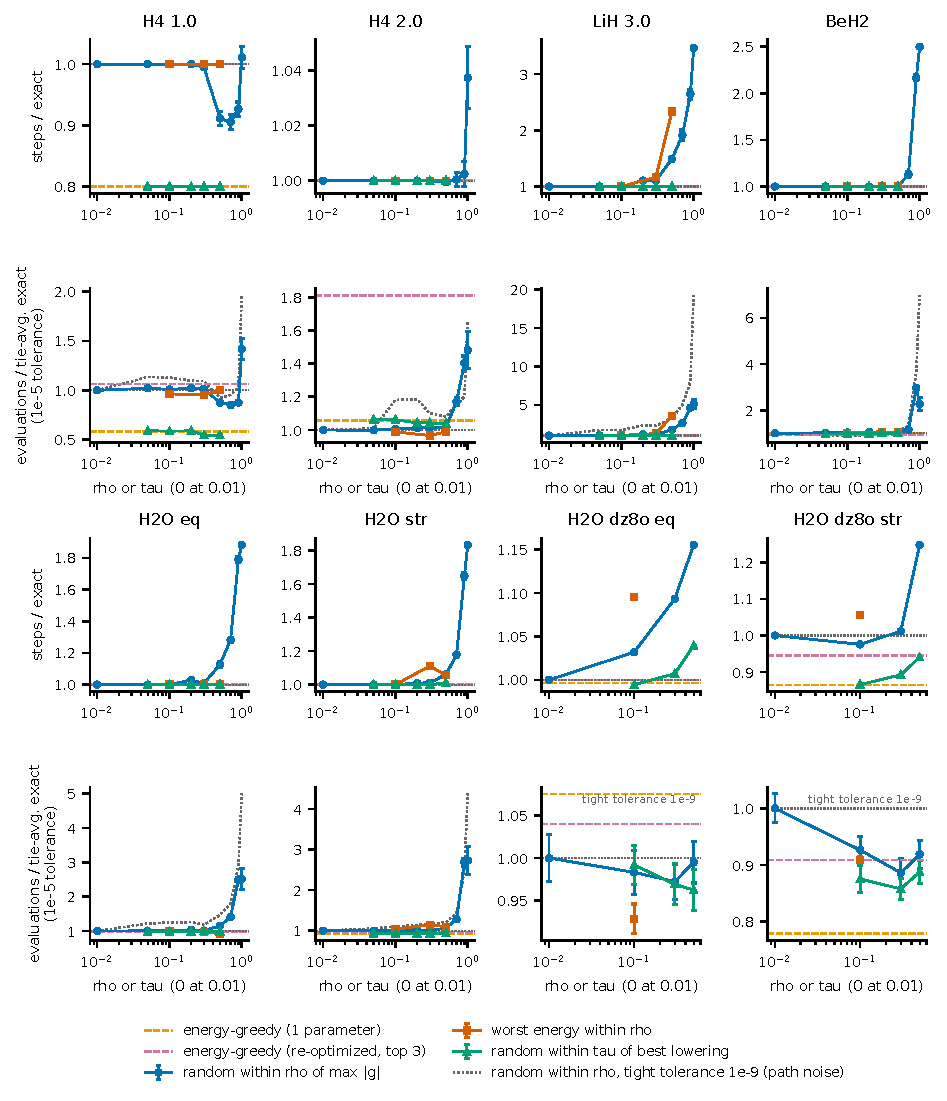
\includegraphics[width=0.92\textwidth]{figures/findings_dose_response.pdf}
  \caption{Dose--response of the selection error. Top: steps over exact ADAPT's (for the 16-qubit windows, where ADAPT does not reach chemical accuracy: energy error after 40 steps over exact ADAPT's) against the tolerance, for a draw inside the gradient set (blue), the worst energy inside it (orange) and a draw inside the
  energy set (green); dashed: energy-greedy references. Bottom: optimizer evaluations over those of random choices among exactly tied generators at the BFGS gradient tolerance $10^{-5}$ (cluster build; dotted: the draw inside the gradient set at the tight tolerance $10^{-9}$, where the count carries the path noise of the polishing, Sec.~\ref{sec:gtol}; the windows were run at $10^{-9}$ only). Error bars: 95\% intervals; 200 trajectories per point (48 for the windows).}
  \label{fig:dose}
\end{figure}

\paragraph{Reading.} (i) The tolerance $\rho^\ast$ up to which the steps stay within $3\%$ depends on the system: $0.1$ on LiH (at $\rho=0.2$ $63\%$ of the trajectories need a seventh step), $0.3$ on H$_2$O, $0.5$ on BeH$_2$, at least $0.9$ on H$_4$ 2.0~\AA. The default $\rho=0.1$ of the paper is the largest value that is harmless on all systems; it is conservative for the others.
(ii) The tolerance on the energy lowering is harmless up to $\tau=0.5$ everywhere (Table~\ref{tab:find_tau}); the gradient is the wrong currency for a tolerance because it does not know the curvature. (iii) A random draw at every step ($\rho=1$) fails (reaches chemical accuracy in $10\%$ of the LiH runs and in none of the BeH$_2$ and H$_2$O runs): the pool is not forgiving enough for arbitrary choices,
so there is a real boundary between harmless and harmful errors, at $\rho\approx0.3$--$0.7$ for the larger pools. (iv) On the 16-qubit window the energy at step 40 is $3\%$ worse at $\rho=0.1$ and $9\%$ at $\rho=0.3$ on the equilibrium geometry and unchanged on the stretched one (Table~\ref{tab:find_window}).
(v) At the tight tolerance the evaluation count rises with $\rho$ already at $0.05$ ($+22\%$ H$_2$O eq, $+73\%$ LiH); at $10^{-5}$ and $10^{-3}$ it does not (Table~\ref{tab:find_rho_evals}): $\rho\le0.1$ costs at most $+5\%$ in evaluations on all six systems, and larger tolerances cost what their extra steps cost ($+14$--$15\%$ at $\rho=0.3$ and $+65$--$76\%$ at $0.5$ on LiH, whose steps grow by $11\%$ and $49\%$): Section~\ref{sec:gtol}.

%==================================================================================================
\section{Is the gradient the right currency?}\label{sec:greedy}

% BEGIN INLINE findings_policies_greedy
\begin{table}[!htb]
\centering\small
\caption{Energy-greedy choices: steps relative to exact ADAPT when every selection is the generator with the largest one-parameter lowering (one-param.), the largest Newton estimate $g_i^2/2h_i$ with the curvature $h_i$ of the Hartree--Fock reference (no shots) or of the current state, or the lowest energy after re-optimizing all parameters among the top 3 / top 10 gradients / all generators with a gradient. Only H$_4$ 1.0~\AA\ gains steps (10 to 8; H$_2$O eq 17 to 16 with all candidates re-optimized). The steps are the same at $10^{-5}$ and $10^{-3}$, except that the H$_2$O eq gain disappears at $10^{-3}$.}
\label{tab:find_greedy}
\footnotesize\setlength{\tabcolsep}{3.5pt}
\fitcol{%
\begin{tabular}{lrrrrrr}
\toprule
System & one-param. & Newton, HF curv. & Newton, exact curv. & re-opt., top 3 & re-opt., top 10 & re-opt., all \\
\midrule
H$_4$ 1.0~\AA & 0.80 & 1.00 & 0.90 & 1.00 & 0.80 & 0.80 \\
H$_4$ 2.0~\AA & 1.00 & 1.00 & 1.00 & 1.00 & 1.00 & 1.00 \\
LiH 3.0~\AA & 1.00 & 1.00 & 1.00 & 1.00 & 1.00 & 1.00 \\
BeH$_2$ & 1.00 & 1.00 & 1.00 & 1.00 & 1.00 & 1.00 \\
H$_2$O eq & 1.00 & 1.00 & 1.00 & 1.00 & 1.00 & 0.94 \\
H$_2$O str & 1.00 & 1.00 & 1.00 & 1.00 & 1.00 & 1.00 \\
\bottomrule
\end{tabular}}
\end{table}
% END INLINE findings_policies_greedy

% BEGIN INLINE findings_policies_window
\begin{table}[!htb]
\centering\small
\caption{Sixteen-qubit cc-pVDZ window of H$_2$O (360 generators, Hartree--Fock start): mean energy error (mHa) after 20 and after 40 ADAPT steps for the choices of the header (48 trajectories for the random ones; exact ADAPT is still at $5.9$ / $3.7$~mHa after 40 steps; the energies of the random choices are means). On the stretched geometry the energy-based choices are lower by $14$\% (step 40) and $24$\% (step 20); on the equilibrium geometry a gradient tolerance of $0.1$ costs $3$\% and $0.3$ costs $9$\% in the energy at step 40, an adversarial choice inside the $\rho=0.1$ set $10$\%.}
\label{tab:find_window}
\footnotesize\setlength{\tabcolsep}{3.5pt}
\fitcol{%
\begin{tabular}{llrrrrrrrrr}
\toprule
System & step & exact & one-param. & Newton HF & re-opt. top 3 & $\tau=0.1$ & $\tau=0.3$ & $\rho=0.1$ & $\rho=0.3$ & $\rho=0.1$, worst \\
\midrule
H$_2$O cc-pVDZ window eq & 20 & 12.75 & 12.69 & 12.69 & 12.70 & 12.72 & 12.84 & 12.86 & 13.14 & 12.89 \\
 & 40 & 5.88 & 5.86 & 5.86 & 5.88 & 5.85 & 5.92 & 6.07 & 6.43 & 6.44 \\
H$_2$O cc-pVDZ window str & 20 & 16.29 & 12.43 & 12.41 & 12.90 & 12.49 & 12.64 & 15.83 & 16.51 & 16.33 \\
 & 40 & 3.74 & 3.23 & 3.21 & 3.53 & 3.24 & 3.34 & 3.65 & 3.78 & 3.95 \\
\bottomrule
\end{tabular}}
\end{table}
% END INLINE findings_policies_window

% BEGIN INLINE findings_rhomap
\begin{table}[!htb]
\centering\small
\caption{What the gradient tolerance guarantees for the energy lowering (HF, CISD and every state of the exact ADAPT trajectory; one-parameter move and full re-optimization after the generator is appended). Top $|g|$ share: lowering of the largest-$|g|$ generator over the best lowering (mean, minimum in brackets). Energy-best in the set: share of states whose best generator has $|g|\ge0.9\max|g|$. Worst $\rho$-good: the worst generator with $|g|\ge0.9\max|g|$ over the best (mean, minimum). Rho needed: $1-|g_\text{best}|/\max|g|$, the tolerance that contains the energy-best generator (median, maximum).}
\label{tab:find_rhomap}
\footnotesize\setlength{\tabcolsep}{3.5pt}
\fitcol{%
\begin{tabular}{lrrrrrrrrr}
\toprule
 & & \multicolumn{4}{c}{one-parameter move} & \multicolumn{4}{c}{after re-optimizing all parameters} \\
\cmidrule(lr){3-6}\cmidrule(lr){7-10}
System & states & top $|g|$ share & energy-best in $\rho=0.1$ set & worst $\rho$-good & rho needed & top $|g|$ share & energy-best in $\rho=0.1$ set & worst $\rho$-good & rho needed \\
\midrule
H$_4$ 1.0~\AA & 11/10 & 0.62 (0.11) & 55\% & 0.52 (0.05) & 0.04 (0.67) & 0.52 (0.08) & 50\% & 0.42 (0.03) & 0.09 (0.67) \\
H$_4$ 2.0~\AA & 11/10 & 0.96 (0.60) & 91\% & 0.89 (0.48) & 0.00 (0.28) & 0.96 (0.60) & 90\% & 0.87 (0.43) & 0.00 (0.28) \\
LiH 3.0~\AA & 6/6 & 1.00 (1.00) & 100\% & 0.98 (0.86) & 0.00 (0.00) & 1.00 (1.00) & 100\% & 0.98 (0.90) & 0.00 (0.00) \\
H$_2$O eq & 18/17 & 0.93 (0.59) & 72\% & 0.83 (0.55) & 0.00 (0.26) & 0.83 (0.45) & 47\% & 0.74 (0.27) & 0.11 (1.00) \\
H$_2$O str & 19/18 & 0.87 (0.32) & 84\% & 0.76 (0.20) & 0.00 (0.24) & 0.82 (0.30) & 61\% & 0.71 (0.19) & 0.04 (0.99) \\
\bottomrule
\end{tabular}}
\end{table}
% END INLINE findings_rhomap

% BEGIN INLINE findings_policies_nrho
\begin{table}[!htb]
\centering\small
\caption{Curvature-scaled tolerance, cluster build, BFGS gradient tolerance $10^{-5}$, 200 trajectories per entry. Each cell is \emph{plain gradient set} / \emph{curvature-scaled set}: the draw is uniform among the generators with $|g_i|\ge(1-R)\max|g|$, respectively with $|g_i|/\sqrt{h_i}\ge(1-R)\max|g_j|/\sqrt{h_j}$, $h_i$ the diagonal curvature at the Hartree--Fock reference (no extra shots). The last column is the draw inside the set of one-parameter energy lowerings within $30\%$ of the best (needs the lowering at every step). The evaluation ratios are relative to the exact path of the same build, as in the preceding tables.}
\label{tab:find_nrho}
\footnotesize\setlength{\tabcolsep}{3.5pt}
\fitcol{%
\begin{tabular}{lrrrrrr}
\toprule
System & $R=0.1$ & $R=0.2$ & $R=0.3$ & $R=0.5$ & $R=0.7$ & $\tau=0.3$ \\
\midrule
\multicolumn{7}{l}{\emph{Steps relative to exact ADAPT}} \\
H$_4$ 1.0~\AA & 1.00 / 1.00 & 1.00 / 1.00 & 0.99 / 0.99 & 0.91 / 0.91 & 0.91 / 0.91 & 0.80 \\
H$_4$ 2.0~\AA & 0.98 / 1.00 & 0.99 / 0.99 & 0.99 / 0.99 & 0.97 / 0.97 & 0.99 / 0.98 & 1.00 \\
LiH 3.0~\AA & 1.00 / 1.00 & 1.11 / 1.00 & 1.11 / 1.11 & 1.49 / 1.12 & 1.91 / 1.30 & 1.00 \\
BeH$_2$ & 1.00 / 1.00 & 1.00 / 1.00 & 1.00 / 1.00 & 1.00 / 1.00 & 1.13 / 1.00 & 1.00 \\
H$_2$O eq & 1.00 / 1.00 & 1.03 / 1.00 & 1.01 / 1.00 & 1.13 / 1.03 & 1.28 / 1.21 & 1.00 \\
H$_2$O str & 1.00 / 0.98 & 1.01 / 1.00 & 1.01 / 1.02 & 1.06 / 1.10 & 1.18 / 1.18 & 1.00 \\
\multicolumn{7}{l}{\emph{Optimizer evaluations relative to exact ADAPT}} \\
H$_4$ 1.0~\AA & 1.01 / 1.00 & 1.02 / 1.01 & 1.01 / 1.01 & 0.88 / 0.87 & 0.85 / 0.85 & 0.55 \\
H$_4$ 2.0~\AA & 1.01 / 1.04 & 1.01 / 1.02 & 1.02 / 1.02 & 1.02 / 1.03 & 1.17 / 1.17 & 1.04 \\
LiH 3.0~\AA & 1.01 / 1.01 & 1.15 / 1.01 & 1.15 / 1.37 & 1.76 / 1.37 & 2.64 / 1.99 & 1.01 \\
BeH$_2$ & 1.04 / 0.98 & 1.06 / 1.00 & 1.05 / 1.01 & 1.03 / 1.02 & 1.16 / 1.03 & 1.00 \\
H$_2$O eq & 1.00 / 0.99 & 1.03 / 0.99 & 1.02 / 0.99 & 1.15 / 1.01 & 1.41 / 1.23 & 0.99 \\
H$_2$O str & 1.00 / 0.90 & 1.00 / 0.92 & 1.00 / 0.92 & 1.06 / 1.01 & 1.28 / 1.13 & 0.93 \\
\bottomrule
\end{tabular}}
\end{table}
% END INLINE findings_policies_nrho


% BEGIN INLINE findings_policies_nrho_window
\begin{table}[!htb]
\centering\small
\caption{The 16-qubit cc-pVDZ windows of H$_2$O at the BFGS gradient tolerance $10^{-5}$ (cluster build, 48 trajectories per random policy, 40 steps). Error: mean energy error after 40 steps over that of exact ADAPT; ``within target'': share of the trajectories ending below the target error of the analysis script (exact ADAPT's own final error plus its tolerance); evaluations relative to exact ADAPT. ``curv.'' is the curvature-scaled gradient set.}
\label{tab:find_nrho_window}
\footnotesize\setlength{\tabcolsep}{3.5pt}
\fitcol{%
\begin{tabular}{llrrrrrrrr}
\toprule
System & quantity & $\rho=0.1$ & curv.\ $0.1$ & $\rho=0.3$ & curv.\ $0.3$ & $\rho=0.5$ & curv.\ $0.5$ & $\tau=0.3$ & one-param. \\
\midrule
H$_2$O cc-pVDZ window eq & error, step 40 & 1.03 & 1.00 & 1.09 & 1.04 & 1.16 & 1.21 & 1.01 & 1.00 \\
 & within target (\%) & 25 & 100 & 4 & 23 & 4 & 0 & 92 & 100 \\
 & evaluations & 0.98 & 0.98 & 0.97 & 0.97 & 0.96 & 0.94 & 0.97 & 1.00 \\
H$_2$O cc-pVDZ window str & error, step 40 & 0.98 & 0.89 & 1.01 & 0.92 & 1.25 & 1.15 & 0.89 & 0.86 \\
 & within target (\%) & 98 & 100 & 60 & 100 & 12 & 23 & 100 & 100 \\
 & evaluations & 0.99 & 0.87 & 0.99 & 0.89 & 1.03 & 0.90 & 0.86 & 0.86 \\
\bottomrule
\end{tabular}}
\end{table}
% END INLINE findings_policies_nrho_window



\paragraph{Reading.} The gradient is the first-order slope at $\theta=0$; the energy lowering after a full step and re-optimization depends on the curvature and on the coupling to the other parameters. Table~\ref{tab:find_rhomap} quantifies the mismatch; it does not translate into a loss of steps on the STO-3G molecules (Table~\ref{tab:find_greedy}), where ADAPT corrects a suboptimal generator later, but it does where the pool is degenerate and small (H$_4$ 1.0~\AA:
the best first generator has a $47\%$ smaller gradient and five times the lowering, 8 steps instead of 10) or large (stretched window: $-24\%$ in the energy at step 20, $-14\%$ at step 40). The Newton estimate $g_i^2/2h_i$ with the curvature of the Hartree--Fock state needs no measurement at run time (the reference is a basis state) and reproduces the gain
of the energy-greedy choice on the stretched window ($3.21$ against $3.23$~mHa) but not on H$_4$ 1.0~\AA\ (10 steps). \emph{Curvature-scaled tolerance} (the $\rho$-set of $|g_i|/\sqrt{h_i}$ with $h_i$ at the HF state, i.e.\ the same elimination on classically rescaled arms; no shots; Tables~\ref{tab:find_nrho}--\ref{tab:find_nrho_window}, cluster build, tolerance $10^{-5}$): the steps stay within $3\%$ of exact ADAPT one grid step further than for the plain gradient set on LiH ($0.2$ against $0.1$; at $0.5$ the steps grow by $12\%$ against $49\%$), on BeH$_2$ ($0.7$ against $0.5$), on H$_2$O eq ($0.5$ against $0.3$) and on the 16-qubit equilibrium window (at $0.1$ all trajectories reach the target against $25\%$; at $0.3$ $23\%$ against $4\%$), and it
reaches the target on the stretched window at $0.3$ ($100\%$ against $60\%$); it gives nothing on H$_4$ (both 1.0 and 2.0~\AA), and on stretched H$_2$O it is the same up to $0.3$ and worse at $0.5$ ($+10\%$ against $+6\%$ in the steps), so the HF curvature is a partial proxy only. At small tolerance it also takes the evaluation-saving choices of the energy-based rules on stretched H$_2$O ($-8$ to $-11\%$ at $0.05$--$0.3$, as for $\tau=0.3$ and the Newton choice) and costs $+37\%$ on LiH at $0.3$ (plain: $+15\%$). It does not reach the energy-lowering set: $\tau=0.3$ keeps the steps of exact ADAPT on every system, and at step 40 it is within $1\%$ of exact ADAPT's energy on the equilibrium window and $11\%$ lower on the stretched one.

%==================================================================================================
\section{Repairing the small-sample intervals at trajectory level}\label{sec:e5}

% BEGIN INLINE findings_e5
\begin{table}[!htb]
\centering\small
\caption{Repairing the small-sample intervals at trajectory level: complete II-A trajectories on LiH 3.0~\AA\ (exact ADAPT: 6 steps), a priori start, $\rho=0.1$, per-round intervals, with the default minimum of 50 shots per fold and with 200 and 400 (the same minimum is the floor of the learned designs). Default: the 90 runs of the main set (seeds 7 and 8). A trajectory is above exact if it needs more steps than exact ADAPT; the extra step is the only effect.}
\label{tab:find_e5}
\footnotesize\setlength{\tabcolsep}{3.5pt}
\fitcol{%
\begin{tabular}{lrrrrrl}
\toprule
Minimum shots per fold & runs & steps & runs above exact & $\rho$-good & exact best & selection shots, mean [95\% CI] \\
\midrule
50 (default) & 90 & 6.056 & 5.6\% & 99.1\% & 92.1\% & $5.16\times10^{7}$ [$4.76\times10^{7}$, $5.59\times10^{7}$] \\
200 & 90 & 6.000 & 0.0\% & 100.0\% & 97.8\% & $5.08\times10^{7}$ [$4.74\times10^{7}$, $5.43\times10^{7}$] \\
400 & 90 & 6.011 & 1.1\% & 99.8\% & 94.6\% & $5.23\times10^{7}$ [$4.93\times10^{7}$, $5.54\times10^{7}$] \\
\bottomrule
\end{tabular}}
\end{table}
% END INLINE findings_e5


\paragraph{Reading.} Q9 of the draft showed that II-A's intervals miss at fixed late states with the default minimum of 50 shots per fold and that a minimum of 200--400 repairs them. At trajectory level the effect of the invalid intervals is small but not zero: on LiH 3.0~\AA\ five of 545 selections ($0.9\%$) are not $\rho$-good, all the same generator ($D\,0,1\to4,5$, shortfall $0.126$--$0.151$, i.e.\ just outside $\rho=0.1$),
at steps 4 and 5 where the selection costs $2\times10^7$--$8\times10^7$ shots, and each costs one extra ADAPT step ($5.6\%$ of the trajectories). On H$_2$O (36 runs per geometry) and H$_4$ (96 runs) every choice of II-A and II-0 was $\rho$-good and the steps are exactly those of exact ADAPT. A minimum of 200 shots per fold removes the extra steps ($0\%$) and costs nothing in selection shots (means
within $\pm3\%$), so it is a free default; a minimum of 400 behaves the same within the sampling error ($1.1\%$).

%==================================================================================================
\section{The optimizer tolerance and the cost model}\label{sec:gtol}

\texttt{AdaptSystem.optimize} converges BFGS to a gradient tolerance of $10^{-9}$ (maximum norm). A gradient estimated from shots cannot resolve that: with energies to 1~mHa a parameter-shift gradient has a standard deviation of $\varepsilon_E/\sqrt2\approx7\times10^{-4}$~Ha/rad, so a stop near $10^{-3}$ is the one that is consistent with the cost model, and chemical accuracy needs far less
(near a minimum with curvature of order one the energy error at $|g|=10^{-3}$ is of the order $10^{-6}$~Ha, and the final energies of the exact path agree to about $10^{-6}$~Ha between $10^{-9}$ and $10^{-3}$; along flat directions it can be much larger, Table~\ref{tab:find_tol_energy}). Table~\ref{tab:find_evals} gives the counts of the exact path in both builds: the evaluations fall by $1.7$--$2.9$ (WSL) and $1.3$--$3.3$ (cluster) times at $10^{-5}$ and by $2.5$--$6.2$ and $1.9$--$5.5$ times at $10^{-3}$, and at both tolerances the two builds give the same count (nine of nine comparisons).

% BEGIN INLINE findings_gtol_paths
\begin{table}[!htb]
\centering\small
\caption{The path dependence of the optimizer cost at the tight tolerance, LiH 3.0~\AA: the same six generators (up to symmetry partners; D: double, S: single, orbital labels as in the pool) added in different orders end at the same energy but need between $54$ and $252$ BFGS evaluations at $10^{-9}$ (cluster build; $83$ or $156$ in the WSL build). At $10^{-5}$ every order, tied or near-tied, needs $39$ or $40$ and at $10^{-3}$ $30$ or $31$ (both builds, 100 and 200 random orders).}
\label{tab:find_gtol_paths}
\footnotesize\setlength{\tabcolsep}{3.5pt}
\fitcol{%
\begin{tabular}{p{6.5cm}lrl}
\toprule
Order of the generators (LiH 3.0~\AA, 6 steps) & choices allowed & runs & evaluations (cluster, $10^{-9}$) \\
\midrule
D10,11 D5,10 D4,11 D4,5 S2$\to$4 S3$\to$11 & tied $|g|$ & 52 & 54 \\
D10,11 D5,10 D4,11 D4,5 S3$\to$5 S2$\to$10 & tied $|g|$ & 56 & 55 \\
D10,11 D4,11 D5,10 D4,5 S3$\to$5 S2$\to$10 & tied $|g|$ & 46 & 115 \\
D10,11 D4,11 D5,10 D4,5 S2$\to$4 S3$\to$11 & tied $|g|$ & 46 & 116 \\
D10,11 D5,10 D4,11 D4,5 S2$\to$4 S3$\to$11 & within 5\% of $\max|g|$ & 30 & 54 \\
D10,11 D5,10 D4,11 D4,5 S3$\to$5 S2$\to$10 & within 5\% of $\max|g|$ & 26 & 55 \\
D10,11 D4,11 D5,10 D4,5 S3$\to$5 S2$\to$10 & within 5\% of $\max|g|$ & 28 & 115 \\
D10,11 D4,11 D5,10 D4,5 S2$\to$4 S3$\to$11 & within 5\% of $\max|g|$ & 18 & 116 \\
D10,11 D5,10 D4,5 D4,11 S3$\to$5 S2$\to$10 & within 5\% of $\max|g|$ & 29 & 177 \\
D10,11 D4,11 D4,5 D5,10 S2$\to$4 S3$\to$11 & within 5\% of $\max|g|$ & 23 & 193 \\
D10,11 D5,10 D4,5 D4,11 S2$\to$4 S3$\to$11 & within 5\% of $\max|g|$ & 23 & 209 \\
D10,11 D4,11 D4,5 D5,10 S3$\to$5 S2$\to$10 & within 5\% of $\max|g|$ & 23 & 252 \\
\midrule
all orders (WSL build) & within 5\% & 100 & 39, 40 at $10^{-5}$; 30, 31 at $10^{-3}$ \\
all orders (cluster build) & within 5\% & 200 & 39, 40 at $10^{-5}$; 30, 31 at $10^{-3}$ \\
\bottomrule
\end{tabular}}
\end{table}
% END INLINE findings_gtol_paths


\paragraph{Path dependence.} At $10^{-9}$ the evaluation count depends on the order in which near-degenerate generators are added, although the final energy is the same (Table~\ref{tab:find_gtol_paths}): the optimizer spends its evaluations polishing the last digits along nearly flat directions. At $10^{-5}$ and $10^{-3}$ the mean over random orders of tied generators equals the count of the exact path to the digit in every system tested, in both builds,
and the orders of near-tied generators ($\rho=0.05$, 200 trajectories) cost at most $+3\%$ on the six systems (Table~\ref{tab:find_rho_evals}; at $10^{-5}$: $+1.3\%$ on LiH, $+0.5\%$ on H$_2$O eq, $+2.1\%$ on H$_4$ 1.0~\AA). Consequently: (a) the tie-order noise in her Tables~2 and 3 and the ``near-tie choices cost $22$--$73\%$ more evaluations'' of the policy experiments at $10^{-9}$ are not properties of the selection; (b) the $+19\%$ of H$_4$ 2.0~\AA\ at 68\% has the same origin: at $10^{-5}$ and $10^{-3}$ it is $+1\%$ and $+2\%$ (Table~\ref{tab:find_conf}); (c) the draft's $\Copt$ (counts at $10^{-9}$) overestimates the optimization cost of the complete runs by $2.1$--$3.8$ times relative to $10^{-5}$ and $2.9$--$8.1$ times relative to $10^{-3}$ (medians of the replays, Table~\ref{tab:find_shares}), and the selection looks less important than it is.

% BEGIN INLINE findings_shares
\begin{table}[!htb]
\centering\small
\caption{Share of the selection in the total cost of the complete runs (II-A, 95\%) when the optimizer stops at a looser BFGS gradient tolerance, measured by replaying the recorded runs (cluster build; selection shots unchanged, medians). The modelled $C_\mathrm{opt}$ of the draft is the $10^{-9}$ column; the energy shots per evaluation are those of the model.}
\label{tab:find_shares}
\footnotesize\setlength{\tabcolsep}{3.5pt}
\fitcol{%
\begin{tabular}{lrrrrrrrr}
\toprule
System & runs & selection (II-A, 95\%) & $C_\mathrm{opt}$, $10^{-9}$ & $10^{-5}$ & $10^{-3}$ & share, $10^{-9}$ & $10^{-5}$ & $10^{-3}$ \\
\midrule
H$_4$ 1.0~\AA & 48 & $1.1\times10^{6}$ & $2.1\times10^{9}$ & $8.8\times10^{8}$ & $5.8\times10^{8}$ & 0.051\% & 0.12\% & 0.19\% \\
H$_4$ 2.0~\AA & 48 & $9.6\times10^{6}$ & $2.1\times10^{9}$ & $7.7\times10^{8}$ & $5.1\times10^{8}$ & 0.46\% & 1.2\% & 1.9\% \\
LiH 3.0~\AA & 24 & $5.1\times10^{7}$ & $8.7\times10^{8}$ & $4.1\times10^{8}$ & $3.0\times10^{8}$ & 5.6\% & 11\% & 14\% \\
H$_2$O eq & 36 & $1.1\times10^{9}$ & $1.2\times10^{11}$ & $3.2\times10^{10}$ & $1.5\times10^{10}$ & 0.89\% & 3.3\% & 6.8\% \\
H$_2$O str & 36 & $2.7\times10^{9}$ & $1.1\times10^{11}$ & $3.0\times10^{10}$ & $1.7\times10^{10}$ & 2.3\% & 8.2\% & 14\% \\
\bottomrule
\end{tabular}}
\end{table}
% END INLINE findings_shares


\paragraph{Effect on the share of the selection.} Replaying the recorded runs at the looser tolerances raises the selection share of II-A at 95\% from $5.6\%$ to $11$--$14\%$ on LiH, from $0.9\%$ to $3.3$--$6.8\%$ on H$_2$O eq, from $2.3\%$ to $8.2$--$14\%$ on H$_2$O str, from $0.46\%$ to $1.2$--$1.9\%$ on H$_4$ 2.0~\AA\ and from $0.05\%$ to $0.12$--$0.19\%$ on H$_4$ 1.0~\AA\ (Table~\ref{tab:find_shares}). The optimization still makes up at least $85\%$ of the total, but ``negligible'' is wrong for LiH and the H$_2$O geometries.
With a still cheaper optimizer (Hessian recycling, coordinate updates: the draft's sampled-optimizer test found $0.12$--$0.46$ of the model's shots) the shares grow further. The statements ``optimization dominates'' and the end-to-end gains of Q7 therefore depend on the optimizer tolerance and on the optimizer, not only on the system; with the replays they can be given as ranges.

% BEGIN INLINE findings_tol_energy
\begin{table}[!htb]
\centering\small
\caption{Change of the final energy when the optimizer stops at a looser gradient tolerance (replay of the recorded choices, run by run, against the same run at $10^{-9}$; cluster build). The certified runs end within a few $\mu$Ha of their tight-tolerance energy; the uncertified runs with poor choices can stop on a plateau where $|g|$ is below the tolerance although the energy is still far above the minimum (H$_4$ 1.0~\AA, $10^{-3}$: eight of the 23 pilot runs that reach chemical accuracy at $10^{-9}$ end $4$--$76$~mHa higher).}
\label{tab:find_tol_energy}
\footnotesize\setlength{\tabcolsep}{3.5pt}
\fitcol{%
\begin{tabular}{lrrrr}
\toprule
tolerance & runs & largest change (mHa) & runs changing by $>0.1$~mHa & of these, H$_4$ 1.0~\AA \\
\midrule
$10^{-5}$, certified and baselines (II-A, II-0, M1, M2) & 1233 & $3.3\times10^{-7}$ & 0 & 0 \\
$10^{-5}$, uncertified pilot budgets & 132 & 7.4 & 2 & 0 \\
$10^{-3}$, certified and baselines (II-A, II-0, M1, M2) & 1233 & 0.015 & 0 & 0 \\
$10^{-3}$, uncertified pilot budgets & 132 & 76 & 11 & 9 \\
\bottomrule
\end{tabular}}
\end{table}
% END INLINE findings_tol_energy


\paragraph{Accuracy at the looser tolerances.} A gradient tolerance bounds the energy error only where the curvature is not small. Replaying the recorded choices (Table~\ref{tab:find_tol_energy}), the $1233$ certified and baseline runs end within $0.015$~mHa of their tight-tolerance energy at $10^{-3}$ (within $4\times10^{-7}$~mHa at $10^{-5}$). Of the $132$ uncertified pilot runs, two end $0.2$ and $7.4$~mHa higher at $10^{-5}$ (the first still at chemical accuracy) and $11$ at $10^{-3}$, nine of them on H$_4$ 1.0~\AA: the optimizer stops on a plateau where $|g|$ is below the tolerance, as an optimizer limited by shot noise would.
A tolerance of $10^{-5}$ is therefore the safe choice for the cost model of an uncertified baseline and $10^{-3}$ the one that matches the shot noise.

%==================================================================================================
\section{Suggested changes to \texttt{draft.tex}}\label{sec:draft}

\begin{description}
  \item[Abstract and introduction.] State the objective as the energy trajectory: shots saved without hurting steps and final energy, with the gradient-based $\rho$-good stop as a means. One sentence of results: errors inside $\rho\le0.1$ do not change the trajectory (any of the five systems), the harmless tolerance is $0.3$--$0.9$ on the larger pools, and a tolerance on the energy lowering is harmless up to $0.5$.
        Replace ``the repeated reoptimization of the circuit parameters dominates our modeled total cost'' by a statement that names the optimizer tolerance and gives the range (selection $0.05$--$14\%$ of the total for II-A depending on system and tolerance; Table~\ref{tab:find_shares}).
        The premium sentence of the abstract (``cheaper than the certified one on the smallest systems by a factor of $7.2$ \dots'') should add that in total shots the certified selection is not dearer (Table~\ref{tab:find_premium}).
  \item[Sec.~II.K (resource accounting), ADAPT trajectories.] Give the BFGS gradient tolerance, state that the evaluation count depends on it (the modelled $\Copt$ of the complete runs falls by a factor of $2.1$--$3.8$ at $10^{-5}$ and $2.9$--$8.1$ at $10^{-3}$) and on the order of near-degenerate generators and on the build at the tight tolerance, and report $\Copt$ at $10^{-5}$ and $10^{-3}$ (Table~\ref{tab:find_shares}), with $10^{-9}$ as an upper bound.
  \item[Q7 (is selection still the bottleneck).] Recompute the table at $10^{-5}$ and $10^{-3}$ with the replays of Tables~\ref{tab:find_shares} and \ref{tab:find_cost_tol}: the selection of II-A is $0.1$--$14\%$ of the total (the optimization still dominates), and the cheaper selection of II-A pays off against II-0 and M2 ($+5$ to $+28\%$ in total on H$_2$O) and against sequential M1 ($1.7$--$4.9$ times). The sensitivity paragraph (Hessian recycling, factor $a$) is the same statement from the other side.
  \item[Confidence-level sweep (wherever the draft lowers $\delta$).] Add Table~\ref{tab:find_conf}: the selection shots fall by a factor of $1.6$--$3.4$ from 99\% to 68\% and the optimization cost does not change ($0.98$--$1.02$ of the top level at $10^{-5}$ and $10^{-3}$); the same sweep at the tight tolerance shows a spurious rise on H$_4$ 2.0~\AA\ that is path noise of the optimizer.
  \item[Q9 (a priori start, uncertainty).] Add the trajectory-level result of Table~\ref{tab:find_e5}: at the default 50 shots the invalid intervals cost one extra step in $5.6\%$ of the LiH trajectories and nothing elsewhere; the minimum of 200 shots removes it at no cost. Recommend 200 as the default; state that the interval misses of the diagnostics table of Q9 almost never become harmful choices.
  \item[Q10 (what certification costs).] Add the total-shot premium (Table~\ref{tab:find_premium}): the selection-only premium of the draft ($7.1$, $6.4$, $2.1$, $1.0$, $0.5$, $0.4$) becomes $0.95$, $0.96$, $1.02$, $0.81$, $0.96$, $0.86$ in total shots at $10^{-5}$ ($0.78$--$1.00$ at $10^{-3}$; $0.54$--$0.93$ at the tight $10^{-9}$, whose intervals are wide) because the adequate uncertified budgets lengthen the trajectories; say that certification is not dearer in total shots and up to $22\%$ cheaper, and quote the steps-only part ($0.86$--$0.96$) as the one that does not depend on the optimizer tolerance. Add the uncertified pilot budgets of Table~\ref{tab:find_cost_tol} that fail (reach $0$--$25\%$) and the loss of adequacy of the fixed budgets on H$_4$ at $10^{-3}$.
  \item[Q11 (sensitivity to the settings).] Add the dose--response (Table~\ref{tab:find_rho}, Fig.~\ref{fig:dose}): $\rho^\ast$ per system and the $\tau$ tolerance; the sensitivity to $\rho$ of the draft is then explained, not only measured. Mention that the stop on the energy lowering is the more faithful tolerance and what it would need (a second-order estimate), as an outlook.
  \item[Q12 (independent checks).] Add the gate of Table~\ref{tab:find_gate} (fast against original statistics) and the replay of recorded runs (final energies to $10^{-13}$~Ha), and the statement that evaluation counts and their ratios to exact ADAPT are not transferable between builds (Table~\ref{tab:find_evals}).
  \item[Discussion/conclusions.] The gradient is a proxy: Table~\ref{tab:find_rhomap} and the energy-greedy results (H$_4$ 1.0~\AA, stretched window). Limits: simulated shots, no noise, STO-3G plus one 16-qubit window, the optimization cost model.
\end{description}

\paragraph{Wording to avoid.} ``Small errors are free'' without the tolerance and the system; any ratio to exact-ADAPT evaluation counts; ``selection is negligible'' without the optimizer tolerance; ``confidence does not affect the optimization cost''.

%==================================================================================================
\section{Open items}\label{sec:open}
\begin{itemize}
  \item Nothing is running: all cluster jobs of the refocus (feature study, policy grid, E5, tolerance jobs) have finished and are synchronized.
  \item Not run: the policy grid on the 16-qubit windows at $10^{-3}$ and the full grid there at $10^{-5}$ (the windows have $\rho=0.1,0.3,0.5$, the curvature-scaled set and $\tau=0.3$ only; minutes on the cluster); the curvature-scaled tolerance at the tight tolerance $10^{-9}$ and with a finer grid between $0.1$ and $0.5$; a measured (second-order) estimate of the energy lowering; a noisy-circuit variant.
  \item Earlier round, finished but not entered in the draft: \texttt{ref3\_minshots\_*}, \texttt{win\_scaling\_dz11o}, \texttt{h2o\_iiE\_s8} and \texttt{s9}; \texttt{win\_scaling\_631g} timed out after 24~h.
\end{itemize}

\appendix
\section{Files and commands}\label{sec:files}
All paths are relative to \path{part2_estimator_design}. The scripts are on branch \texttt{part2}.
\begin{itemize}
  \item Her scripts (extracted unchanged from \path{h2o_feature_tables_cluster.ipynb}; one audit change in \path{features_ci_sweep.py}): \path{scripts/features_ci_sweep.py}, \path{features_energy_lowering.py}, \path{features_gradient_correlation.py},
        \path{features_replay.py}, \path{features_report.py}, \path{features_figures.py}, \path{src/fastpath.py}. Our checks: \path{features_check_fastpath.py}, \path{features_compare_tzs.py}, \path{features_compare_stats.py}, \path{features_merge.py}, \path{features_regtol.py}.
  \item Policy experiments: \path{scripts/energy_trajectory_policies.py} (policies \texttt{exact}, \texttt{rho\_random:R}, \texttt{rho\_worst\_g:R}, \texttt{rho\_worst\_e:R}, \texttt{tau\_random:T}, \texttt{nrho\_random:R}, \texttt{onep\_greedy}, \texttt{newton\_hf}, \texttt{newton\_exact},
        \texttt{reopt\_top:M}, \texttt{reopt\_all}; option \texttt{--gtol}); report \path{energy_policies_report.py}; tests \path{tests/test_energy_policies.py}.
  \item Analyses: \path{energy_cost_curves.py} (Table~\ref{tab:find_cost}, Fig.~\ref{fig:cost}), \path{energy_conf_noninferiority.py} (Table~\ref{tab:find_conf}), \path{energy_rho_map.py} (Table~\ref{tab:find_rhomap}), \path{energy_e5_compare.py} (Table~\ref{tab:find_e5}),
        \path{energy_findings_tables.py} (all tables of this report).
  \item Data: \path{runs/features} (her layout, with \path{report/}), \path{runs/features_ext} (48 / 24 trajectories per level), \path{runs/features_check}, \path{runs/features_q10} (replays of the recorded Q10 runs; \path{runs/features_q10_gtol1e-5} and \path{..._gtol1e-3}: the same at the looser tolerances), \path{runs/energy_policies_gtol1e-5_cl}, \path{..._gtol1e-3_cl}, \path{runs/features_gtol*_cl} and \path{runs/features_ext_gtol*_cl} (tolerance jobs on the cluster), \path{runs/energy_policies/<case>/policy_*.jsonl}
        with \path{report/}, \path{runs/LiH_R3p0_HF/phase4/*minshots*}.
  \item Regenerate: run \path{scripts/energy_findings_tables.py}, then \path{scripts/paper_a_inline.py} with the option \texttt{--draft} \path{../reports/energy_trajectory_findings.tex}.
\end{itemize}

\end{document}
